%----------------------------------------------------------------------------------------
%	PACKAGES AND OTHER DOCUMENT CONFIGURATIONS
%----------------------------------------------------------------------------------------


\documentclass[fleqn,10pt]{SelfArx} % Document font size and equations flushed left

%----------------------------------------------------------------------------------------
%	COLUMNS
%----------------------------------------------------------------------------------------

\setlength{\columnsep}{0.55cm} % Distance between the two columns of text
\setlength{\fboxrule}{0.75pt} % Width of the border around the abstract
\usepackage{enumitem} % For spacing in enumerate

%----------------------------------------------------------------------------------------
%	COLORS
%----------------------------------------------------------------------------------------

\usepackage[table,xcdraw]{xcolor} % For colored tables. Also NECESSARY for .cls
\definecolor{color1}{RGB}{0,0,90} % Color of the article title and sections
\definecolor{color2}{RGB}{0,20,20} % Color of the boxes behind the abstract and headings
\definecolor{lightgray}{gray}{0.9} % For long table
\definecolor{headcolor}{HTML}{E2F1F3} % For header

%----------------------------------------------------------------------------------------
%	HYPERLINKS
%----------------------------------------------------------------------------------------

\usepackage{hyperref} % Required for hyperlinks
\hypersetup{hidelinks,colorlinks,breaklinks=true,urlcolor=color2,citecolor=color1,linkcolor=color1,bookmarksopen=false,pdftitle={Title},pdfauthor={Author}}

%----------------------------------------------------------------------------------------
%	ARTICLE INFORMATION
%----------------------------------------------------------------------------------------

\JournalInfo{\ } % Journal information
\Archive{} % Additional notes (e.g. copyright, DOI, review/research article)

\PaperTitle{Eavesdropping on and Emulating MIFARE Ultralight and Classic Cards Using Software Defined Radio} % Article title

\Authors{Ilias Giechaskiel\textsuperscript{1}} % Authors
\affiliation{\textsuperscript{1}\textit{CDT in Cyber Security, University of Oxford, Oxford, United Kingdom}} % Author affiliation

\Keywords{} % Keywords - if you don't want any simply remove all the text between the curly brackets
\newcommand{\keywordname}{Keywords} % Defines the keywords heading name

%----------------------------------------------------------------------------------------
%	TABLES
%----------------------------------------------------------------------------------------

\usepackage{longtable}
\newcommand{\specialcell}[2][l]{%
  \begin{tabular}[#1]{@{}l@{}}#2\end{tabular}}

\let\oldlongtable\longtable
\let\endoldlongtable\endlongtable
\renewenvironment{longtable}{\rowcolors{2}{white}{lightgray}\oldlongtable} {
\endoldlongtable}


%----------------------------------------------------------------------------------------
%	MISC
%----------------------------------------------------------------------------------------

\usepackage{subcaption}
\newcommand{\ms}{\ensuremath{\mu s} }


%----------------------------------------------------------------------------------------
%	ABSTRACT
%----------------------------------------------------------------------------------------

\Abstract{
In this report, we describe a Software-Defined Radio (SDR) approach for eavesdropping on Near Field Communications (NFC) and Radio Frequency Identification (RFID) cards operating at 13.56 MHz. We show that GNU Radio and Python make a great platform for prototyping, while maintaining sufficient performance for passive attacks without extensive optimizations and using only modest processing power. We successfully eavesdrop on real MIFARE Ultralight and Classic 1K cards by capturing the raw radio waves with a home-made antenna. We recover the plaintext of both reader and tag fully by demodulating the incoming radio waves, parsing individual bits and error detection codes into packets, and then decrypting them when necessary. On the transmission side, we achieve full software emulation of the reader and of MIFARE Ultralight and Classic 1K cards (including encryption), and partial hardware emulation, where we correctly modulate the signal, but not within the strict timing limits of the protocol. Our transmissions can also be used to prevent legitimate communication by interfering with the intended reader or tag signals.
}


\begin{document}

%----------------------------------------------------------------------------------------
%	TITLE PAGE
%----------------------------------------------------------------------------------------

\flushbottom % Makes all text pages the same height

\maketitle % Print the title and abstract box

%\tableofcontents % Print the contents section

\thispagestyle{empty} % Removes page numbering from the first page

%----------------------------------------------------------------------------------------
%	INTRODUCTION
%----------------------------------------------------------------------------------------

\section{Introduction}
\label{sec:introduction}

Contactless cards and tags have become very popular in recent years, with everyday applications including e-passports \cite{epassports}, ticketing \cite{mbta, chipkaart, classicvulnerabilities}, access control \cite{imperial}, and payment \cite{relay, practicalrelay} systems. However, as these devices operate wirelessly, adversaries can pick up the radio signals and eavesdrop on the communication between a tag and a reader. Traditionally, such attacks on radio communications required dedicated hardware for particular frequencies and modulation types, but with the advent of Software-Defined Radio (SDR), it is possible to use generic equipment and perform the demodulation in software. Even so, despite a range of embedded devices and Field-Programmable Gate Arrays (FPGAs) that are capable of various attacks on Near Field Communication (NFC), Radio Frequency Identification (RFID), and related technologies, to the best of our knowledge no open-source SDR implementation exists for High-Frequency (HF) NFC.\footnote{Though they exist for UHF Gen2 cards. See \url{https://github.com/brunoprog64/rfid-gen2} and \url{https://github.com/yqzheng/usrp2reader} for instance.} 


To this end, we developed such an implementation on an Ettus Research Universal Software Radio Peripheral (USRP) using Python and GNU Radio with an antenna made out of simple wire that allows passive eavesdropping on reader-tag communication. Though our implementation is easily extensible, we focused on MIFARE cards by NXP Semiconductors, since MIFARE has ``a market share of more than 77\% in the transport ticketing industry", with ``150 million reader and 10 billion contactless and dual interface IC's sold" \cite{mifare}. Specifically, we use Ultralight \cite{ultralight} and Classic 1K \cite{classic1k} cards, as the former does not employ any encryption, while the latter uses a broken cryptographic algorithm (Section \ref{subsec:crypto1}), making them ideal candidates for such exploration. Moreover, we achieve full software and partial hardware reader and tag emulation, that can also be used to jam signals between a legitimate tag and reader. In summary, our contributions are as follows:

\begin{enumerate}[noitemsep]
\item We implement in pure Software-Defined Radio a demodulator for NFC/RFID readers and tags operating in the 13.56 MHz frequency, which decodes radio waves into plaintext packets.
\item We test our implementation by eavesdropping on real MIFARE Classic 1K and Ultralight communications with an RFID reader using a home-made antenna and a USRP, successfully decoding any encrypted packets.
\item We additionally implement in software the emulation of both readers and tags, including encryption if necessary.
\item Though our transmission capabilities cannot keep up with the strict timing requirements of the protocol, we show how our implementation can jam real reader-tag communications and prevent the successful transmission of data.
\item Overall, our work shows that prototyping using Software-Defined Radio is sufficient in practice for passive attacks, without the need for extensive optimizations or heavy computing power.
\end{enumerate}

PAPER STRUCTURE


%----------------------------------------------------------------------------------------
%	LITERATURE REVIEW
%----------------------------------------------------------------------------------------

\section{Related Work}
\label{sec:related}

Early work on RFID Hacking was conducted in a non-academic context, and focused on finding vulnerabilities in access control systems \cite{ccc, mbta}. Later,  Buettner and Wetherall \cite{sdruhf, gen2usrp, phymac} experimented more systematically with RFID and SDR, but focused primarily on Gen 2 cards operating at 900 MHz. Their work was extended by others, typically in the context of proposing better protocols \cite{gnuradio, zoe}, but still for Ultra High Frequencies (UHF), with the exception of a recent work by Hassanieh et al. \cite{randomization}, which also included an extension to HF.  

There have also been a number of designs which use microcontrollers and Field-Programmable Gate Arrays (FPGAs) for signal processing, such as the Proxmark 3 \cite{proxmark}, and RFIDler \cite{rfidler}. Though such projects allow the use of custom firmware for additional functionality, they also require dedicated hardware in their design.

The MIFARE Classic cryptographic protocol was reverse-engineered by Nohl et al. by dissolving the plastic surrounding the chips, recovering the individual logic gates and converting them to a high-level algorithm \cite{crypto1}. Garcia et al. then discovered additional vulnerabilities of the protocol based on its nested authentication and parity bits \cite{classicvulnerabilities}. Due to the wide range of applications of the MIFARE Classic, the topic became very popular for Master's thesis projects \cite{classicimplementation, chipkaart, classicrng, imperial}, which found additional vulnerabilities, or examined the problem within the context of a specific application.

Finally, given the widespread availability of NFC-enabled mobile devices, researchers have also focused on NFC relay attacks using mobile phones \cite{relay, practicalrelay}, as well as exploring \cite{nfcsurface} and protecting \cite{engarde} the NFC mobile phone stack. 



%----------------------------------------------------------------------------------------
%	THEORY
%----------------------------------------------------------------------------------------

\section{Background}
\label{sec:background}

The terms Radio Frequency Identification (RFID), Near Field Communication (NFC), contactless smartcards, proximity cards and vicinity cards are often used interchangeably, but they are covered by different standards and concern different parts of the radio spectrum. In this project, we looked at the ISO/IEC 14443 standard, with physical characteristics defined in \cite{iso144431}, modulation and encoding in \cite{iso144432}, initialization and anticollision in \cite{iso144433} and transmission protocols in \cite{iso144434}.

Specifically, we focus on {\bf Type A} communications, whose {\bf carrier frequency} is $f_c=13.56$ MHz. The reader -- or {\bf Proximity Coupling Device (PCD)} -- communicates with the card -- or {\bf Proximity Integrated Circuit Card (PICC)} -- through {\bf 100\% Amplitude Shift Keying (ASK)}, with data using the {\bf Modified Miller} encoding. The communication from tag to reader utilizes {\bf Load Modulation} with a {\bf subcarrier frequency} of $f_s=f_c/16=847.5$ kHz, using {\bf Manchester Encoding}, and both transmit at a rate of 106 kbit/s. 

Because the carrier frequency is $f_c=13.56$ MHz, the wavelength is $c/f_c\approx22$ meters, making it impossible to deploy antennas that would fit in a card-size form-factor. Additionally, because the cards are {\bf passive} (i.e. do not have their own power source), both the communication and the power source are achieved through {\bf inductive coupling} from the PCD's antenna loop to the PICC's antenna loop.  

SECTION STRUCTURE

\subsection{PCD Transmissions}
\label{subsec:pcd}

Amplitude Shift Keying (ASK) of depth $X$\% is a form of digital modulation which specifies that if the amplitude of the signal representing a digital $1$ is equal to $A$ and the amplitude of the signal representing a digital $0$ is equal to $B$, then $X=\frac{A-B}{A+B}$, as showing in Figure \ref{fig:ask}. Specifically, for 100\% ASK, no signal is sent at all during a digital $0$, indicating that such periods must be very brief, since the PICC needs to keep charge (using a capacitor) for the period of silence.

\begin{figure}[h]
  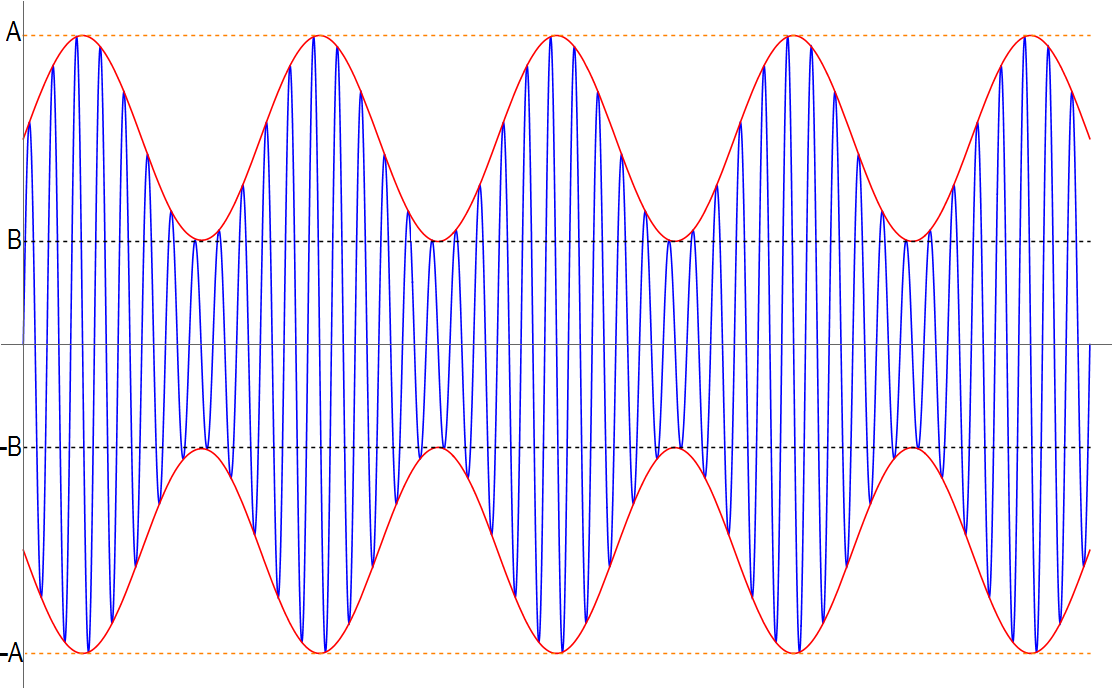
\includegraphics[width=\linewidth]{img/ask}
  \caption{Amplitude Shift Keying (ASK) \cite{atmel}}
  \label{fig:ask}
\end{figure}

This is achieved through the Modified Miller Encoding, which ensures that there is no period of more than 3\ms of silence (``pause"). Specifically, every bit is represented as a (combination of) signals lasting a total of $t_b=128/f_c\approx9.44\ms$. The encoding (show in Figure \ref{fig:miller}) is as follows:
\begin{itemize}[noitemsep] 
\item A 1 is encoded as an unmodulated signal for $t_b/2\approx 4.72 \ms$, followed by a period of silence for 3\ms, followed by an unmodulated signal for $t_b/2-3\approx 1.72\ms$
\item A 0 after a 0 is encoded as a silence period for 3\ms followed by an unmodulated signal for $t_b-3\approx 6.44\ms$
\item A 0 after a 1 is encoded as an unmodulated signal for a period of $t_b\approx9.44\ms$
\item To indicate the beginning and the end of a transmission, a logical 0 is used for both the start and the end
\end{itemize}

\begin{figure}[h]
  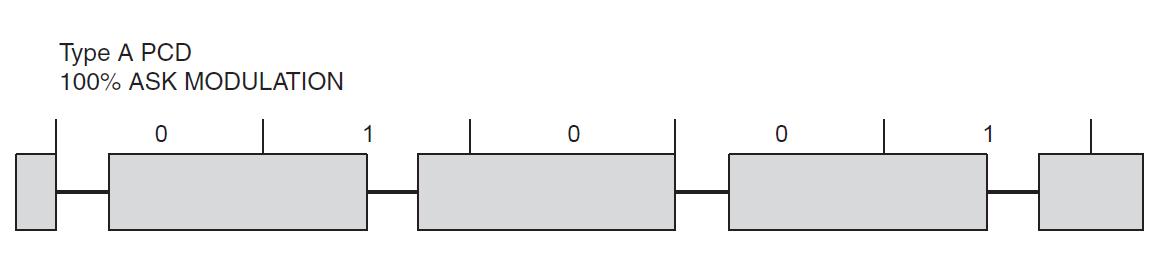
\includegraphics[width=\linewidth]{img/miller}
  \caption{Miller Encoding at 100\% ASK \cite{atmel}}
  \label{fig:miller}
\end{figure}

In practice, however, because of hardware imperfections, the pause is not perfect, but needs to comply with the requirements shown in Figure \ref{fig:pause}. As a result, the modulated carrier for the encodings resembles Figure \ref{fig:miller2}.

\begin{figure}[h]
  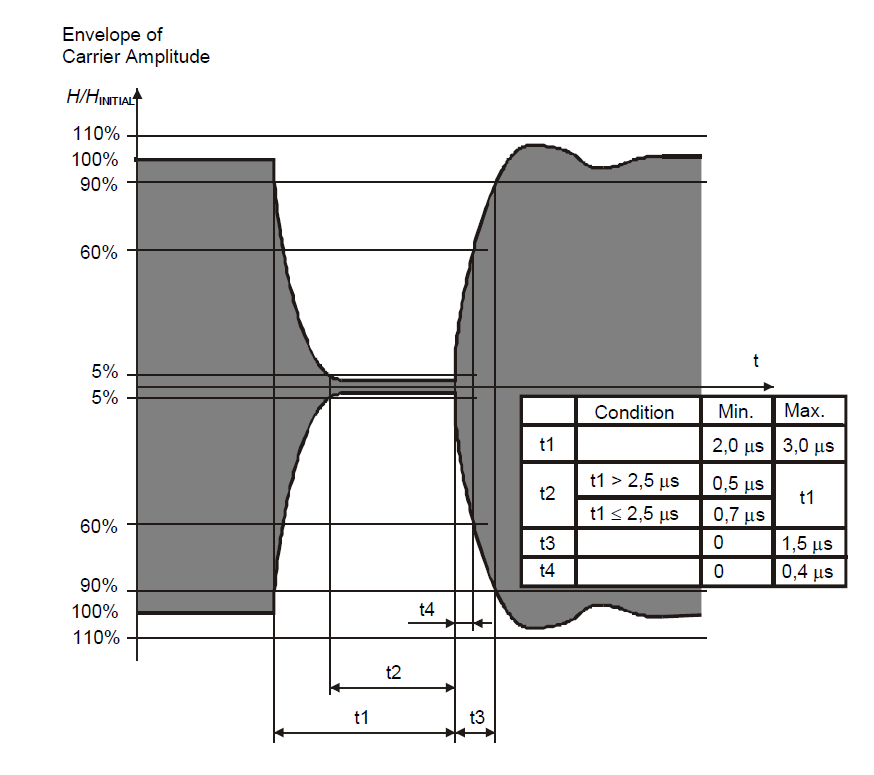
\includegraphics[width=\linewidth]{img/pause}
  \caption{Real Pause Requirements \cite{iso144432}}
  \label{fig:pause}
\end{figure}


\begin{figure}[h]
  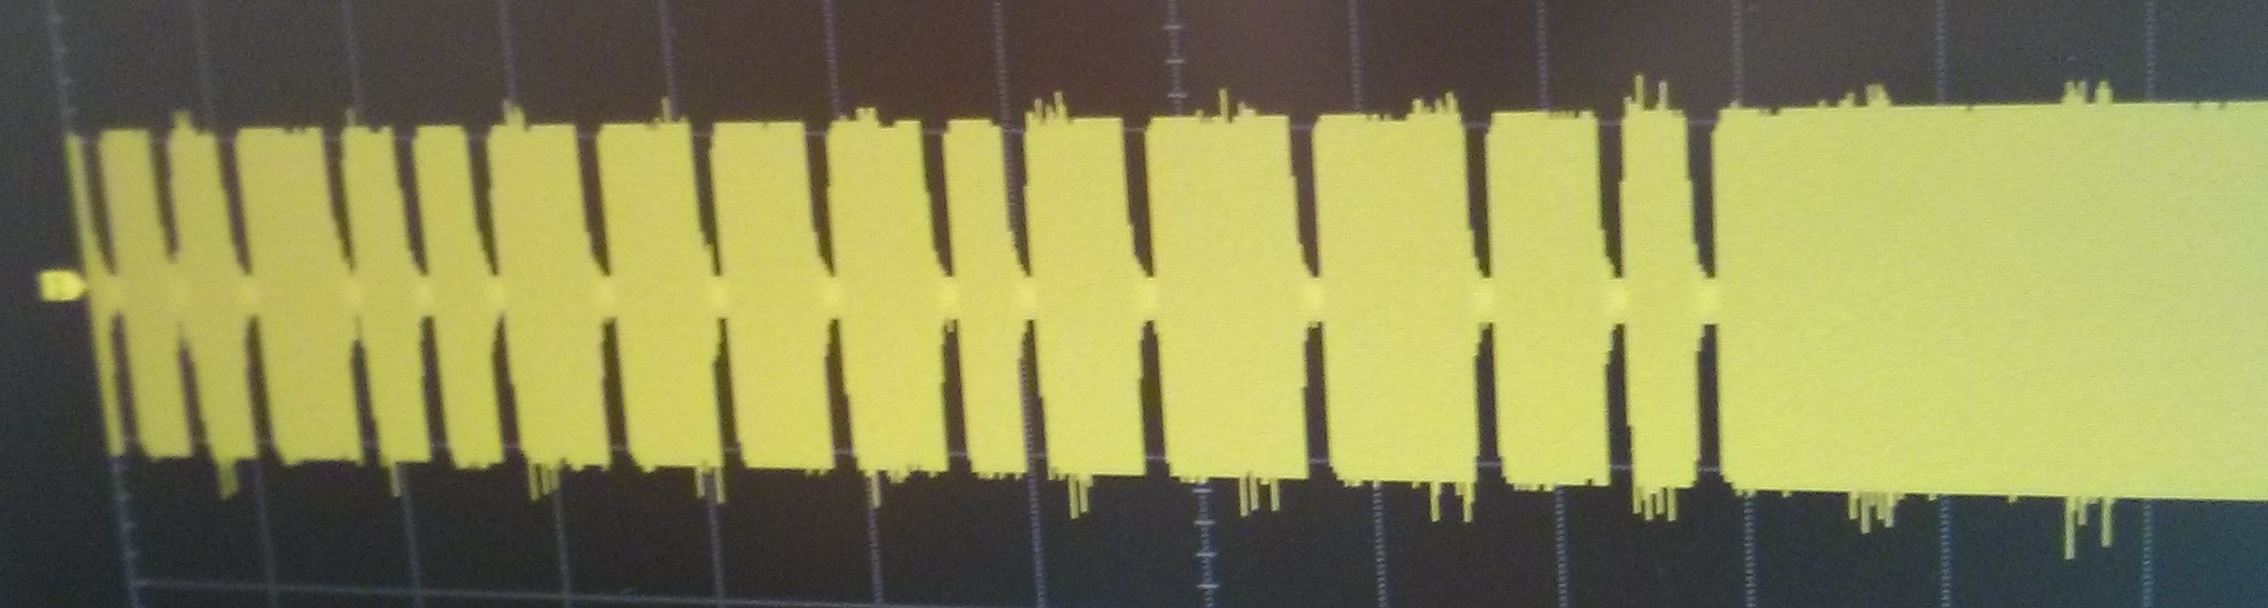
\includegraphics[width=\linewidth]{img/miller2}
  \caption{Realistic Miller Encoding \cite{mifare}}
  \label{fig:miller2}
\end{figure}

\subsection{PICC Transmissions}
\label{subsec:picc}

As mentioned above, the tag does not have sufficient power for active transmissions. Consequently, the PICC achieves data transmission passively, by changing its {\em load}, which can be inferred as a voltage drop on the PCD, hence the term {\bf load modulation}. Switching the load generates a {\bf subcarrier}, which has a frequency $f_s=f_c/16=847.5$ kHz. 

The bits are then encoded using {\bf On-Off Keying (OOK)} or {\bf Manchester Encoding} as follows, with a total duration also equal to $t_b\approx9.44\ms$, which also equals 8 periods of the subcarrier, also shown in Figures \ref{fig:manchester} and \ref{fig:manchester2}:

\begin{itemize}[noitemsep] 
\item A 1 is encoded by modulating the subcarrier for the {\em first} half ($=t_b/2\approx4.72\ms$) of the bit duration
\item A 0  is encoded by modulating the subcarrier for the {\em second} half ($=t_b/2\approx4.72\ms$) of the bit duration
\item A logical 1 starts the transmission
\item No modulation signifies the end of a transmission
\end{itemize}


\begin{figure}[h]
  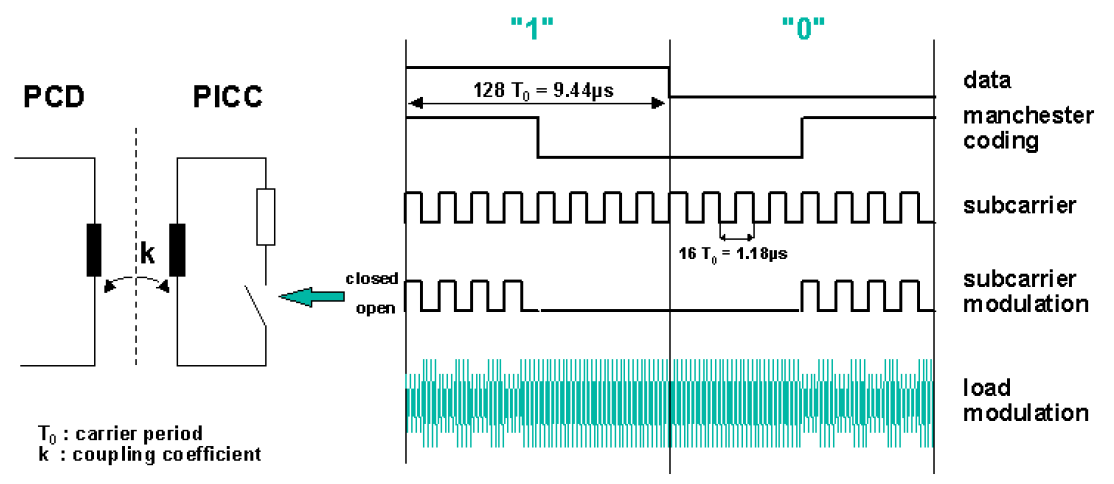
\includegraphics[width=\linewidth]{img/manchester2}
  \caption{Manchester Encoding with Load Modulation \cite{mifare}}
  \label{fig:manchester}
\end{figure}

\begin{figure}[h]
  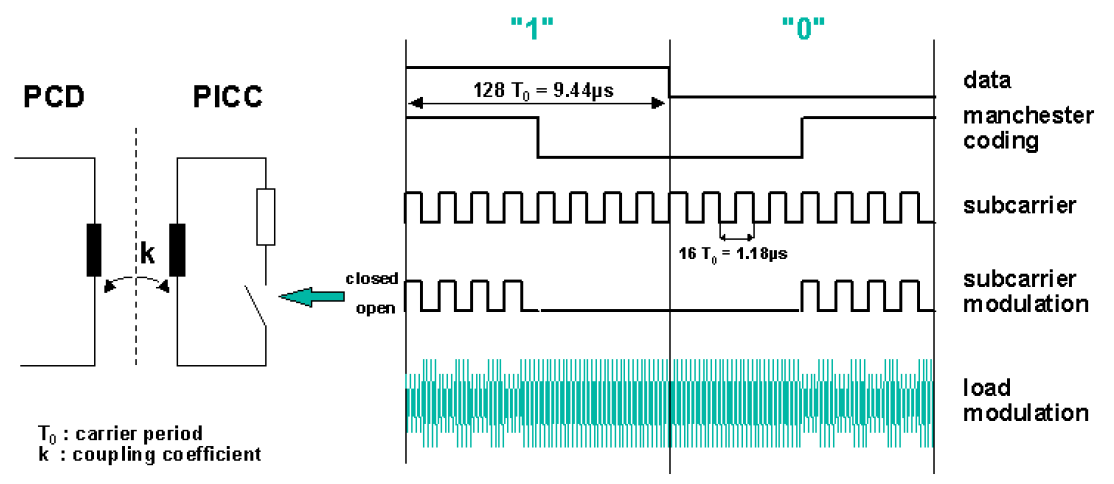
\includegraphics[width=\linewidth]{img/manchester}
  \caption{Envelope of Load Modulation \cite{atmel}}
  \label{fig:manchester2}
\end{figure}

\subsection{The Protocol}
\label{subsec:protocol}

Though the ISO/IEC 14443A protocol is general, we will focus on a few key aspects that are relevant to our discussion. As a result, we will refer the reader to \cite{iso144433} for more details such as timing requirements.

First of all, it is worth noting that each byte is {\bf ordered} from the Least Significant Bit (LSB) to the Most Significant Bit (MSB), and that each byte is followed by an {\bf odd parity bit}, meaning that an even number of high bits (ones) is followed by another high bit (one), whereas an odd number of ones is followed by a low bit (zero). For example, the byte 0x3F is encoded as $1111\ 1100\ 1$.

The PCD signifies that it is waiting to read tags by repeatedly sending a {\bf REQA (0x26)} or a {\bf WUPA (0x52)}, where the ``A" signifies that type A protocol is used. The difference between the REQA request and the WUPA wake-up request is that the latter also wakes up PICCs that were previously asked to HALT. Unlike all other commands, they are sent using a {\em short frame} that only consists of 7 bits, and which does not include a parity bit. As a result, the REQA command (including the beginning and end transmission zero bits) is sent as the sequence of bits $0\ 0110\ 010\ 0$.

The standard has also defined {\bf Anticollision} and {\bf Selection} phases before the transmission of actual data which are used to ensure the non-interference from multiple tags and the correct selection of the tag. However, we only discuss them in the context of the MIFARE cards in Appendix \ref{app:mifare}, since they are not necessary for understanding the rest of this report. 

Finally, we mention that to detect errors with longer transmissions, for some requests and responses a {\bf Cyclic Redundancy Check (CRC)} is used on the transmitted bytes (but excluding start/end and parity bits). The polynomial used is $x^{16}+x^{12}+x^5+1$, with a starting value of 0x6363, under the assumption that ``FF0 shall be the leftmost flip-flop where data is shifted in  [and] FF15 shall be the rightmost flip-flop where data is shifted out" \cite{iso144433}. For example, the {\bf HALT/HLTA} command uses 2 bytes (0x50 0x00) followed by the two CRC bytes which can be calculated as 0x57 0xCD.

\subsection{MIFARE Classic 1K Encryption}
\label{subsec:crypto1}

Even though the MIFARE Ultralight is ISO/IEC 14443 A compliant \cite{ultralight}, the MIFARE Classic 1K uses a proprietary cryptographic protocol called CRYPTO1 \cite{classic1k}. The details of the protocol were not made publicly available, with the MIFARE datasheets only broadly explaining the 3-pass protocol \cite{classic1k}. Each {\bf sector} (equal to 4 {\bf blocks} of 16 bytes each) has two 6-byte keys ({\bf Key A and B}), which on delivery are set to [0xFF 0xFF 0xFF 0xFF 0xFF 0xFF] (but can be changed later on a per-sector basis). Each authentication happens with one of the two keys chosen by the reader, and can only be used to access a specific sector. Each sector contains one block (the {\bf sector trailer}) which contains the two keys and some {\bf access bits} which determine the allowed operations for the 4 blocks (See Appendix \ref{app:classic1k} for more details).


The PCD indicates to the PICC that it wants to authenticate through a command indicating which key to be used and what address to use. As shown in Figures \ref{fig:auth1} and \ref{fig:auth2}, the three-pass scheme consists of a 4 byte challenge sent from the PICC to the PCD  (Token RB), an 8-byte challenge and response (of 4 bytes each) send from the PCD to the PICC (Token AB) and a response from the PICC to the PCD (Token BA), if the reader's encryption was correct. After the first challenge (Token RB), {\bf all} traffic is encrypted, even subsequent authentications, which leads to a weakness known as {\bf nested authentication} \cite{classicvulnerabilities}.

\begin{figure}[h]
  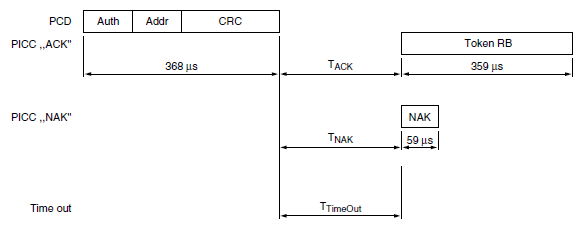
\includegraphics[width=\linewidth]{img/auth1}
  \caption{First Part of Authentication \cite{classic1k}}
  \label{fig:auth1}
\end{figure}

\begin{figure}[h]
  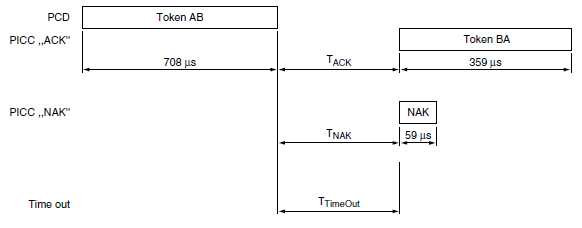
\includegraphics[width=\linewidth]{img/auth2}
  \caption{Second Part of Authentication \cite{classic1k}}
  \label{fig:auth2}
\end{figure}

Though we discuss the encryption algorithm in greater detail in Appendix \ref{app:crypto1}, it is worth noting a few things based on the research in \cite{crypto1, classicvulnerabilities}. The CRYPTO1 encryption scheme is a stream cipher which consists of a 48-bit (equal to the key length) Linear Feedback Shift Register (LFSR) and a non-linear {\bf filter} function \cite{crypto1}. The encryption incorporates both the tag's Unique Identifier (UID) and the random nonce RB, which however is only generated using a 16-bit LFSR. Nonetheless, both challenge responses only depend on the tag's nonce (and not the reader's nonce or the UID), and use the same LFSR as the Random Number Generator (RNG). 

What is more, the parity bits are also encrypted (making the MIFARE Classic 1K {\em incompatible} with the ISO 14443 protocol), and ``the bit of keystream used to encypt the parity bits is reused to encrypt the next bit of plaintext" \cite{classicvulnerabilities}. This vulnerability, in combination with the nested authentication mentioned above (which causes the token RB to also be encrypted) leaks data which can be used to guess the nonce or to reveal the secret key.


%----------------------------------------------------------------------------------------
%	IMPLEMENTATION
%---------------------------------------------------------------------------------------- 

\section{Implementation}
\label{sec:implementation}

SECTIONS


\subsection{Setup and Methodology}

For this project, we used Ettus Research's Universal Software Radio Peripheral (USRP) N210 \cite{usrp}, in combination with the BasicRX/TX and LFRX/TX daughterboards \cite{daughterboards}, both of which cover the 13.56 MHz frequency. The USRP has become the de-facto SDR platform in combination, and also allows custom code to be written on its FPGA, which we did not pursue in this project. Instead, all signal processing was done on a laptop, using Python and the GNU Radio toolkit/framework, which is easily extensible and provides many building blocks (``modules") that can be incorporated into new designs.

For lack of a better alternative, the laptop used is a Samsung NP900X4C with an Intel i5-3317U @ 1.7 GHz and 8 GB of RAM, but the operating system used (Kali Linux 1.1.0a) was booted off a 16 GB USB 3.0 Lexar JumpDrive. Moreover, due to the lack of an Ethernet port, the USRP was connected to the laptop on a Plugable USB3-E1000 USB 3.0 Gigabit Ethernet Adapter.


To measure signals accurately, we used a Rigol DS2302A digital oscilloscope with two 300 MHz channels \cite{rigol}. 

The actual reader was an RFID-RC522 module using the MFRC522 chip by NXP Semiconductors \cite{mfrc522} connected to an Arduino UNO using the Serial Peripheral Interface (SPI) and the DumpInfo example at \cite{library}. A schematic is found in Figure \ref{fig:rc522schematic}, while Figure \ref{fig:rc522pic} is a picture of the module, where the test pad for the reception (RX) part of the antenna is highlighted.


\begin{figure}[h]
  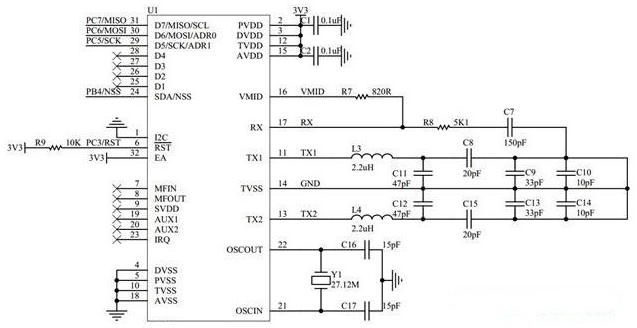
\includegraphics[width=\linewidth]{img/rc522schematic}
  \caption{RC522 Schematic \url{http://img.alibaba.com/img/pb/082/266/824/824266082_485.jpg}}
  \label{fig:rc522schematic}
\end{figure}

\begin{figure}[h]
  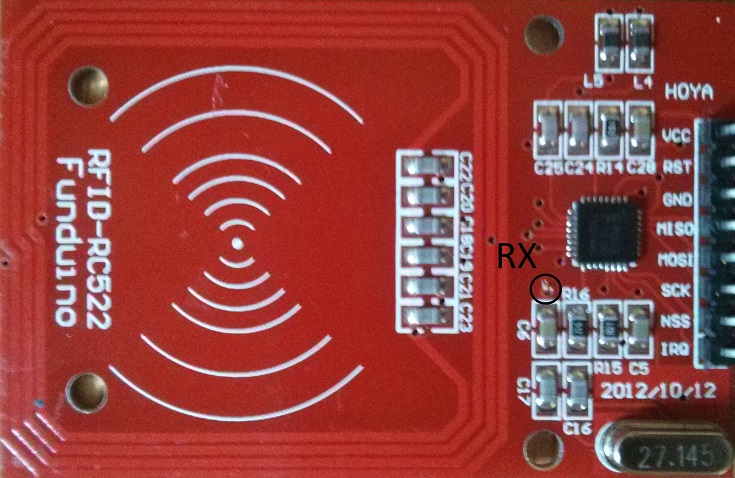
\includegraphics[width=\linewidth]{img/rc522pic}
  \caption{RC522 RX Test Pad}
  \label{fig:rc522pic}
\end{figure}


The types of tags/cards used are shown in Figure \ref{fig:cards} and are a Classic 1K card, and an NTAG203 \cite{ntag203}, which is compatible with the Ultralight. The NTAG203 is actually larger and has a different memory layout, but the Arduino library used does not distinguish between the two, so only 16 out of the 42 pages are revealed. It is important to note that although we only two {\em types} of cards were used, more than one actual card per type was tried with identical results.

\begin{figure}[h]
  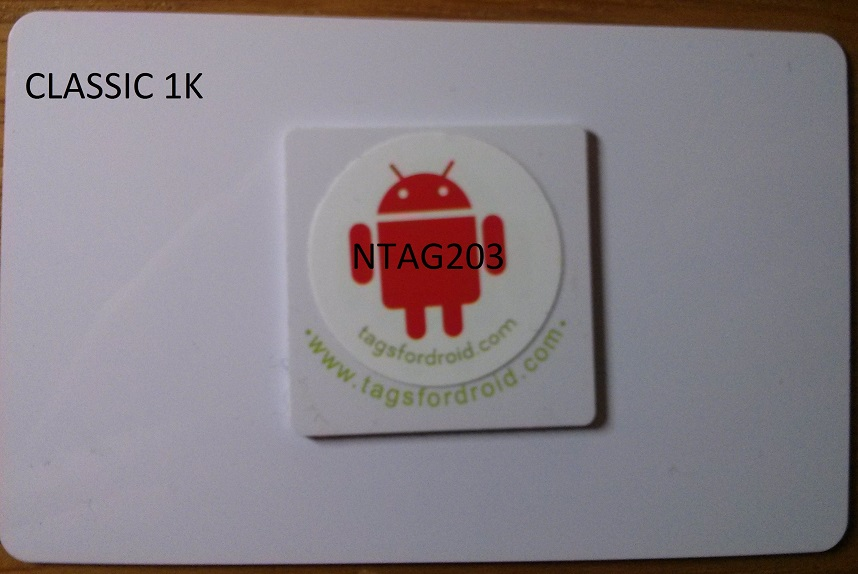
\includegraphics[width=\linewidth]{img/cards}
  \caption{Cards/Tags used for the experiment}
  \label{fig:cards}
\end{figure}

\subsection{The Antenna}
\label{subsec:antenna}

Much research has been conducted into making RFID-type antennas work well and with up to a large distance, with much of it available as application notes \cite{mifare, antenna, pnantenna}. Many of them are also available for direct purchase, such as the DLP-RFID-ANT by DLP Design,\footnote{Found at \url{http://www.dlpdesign.com/rf/ant1.shtml}} but fundamentally the RFID antenna is just an inductor, made out of wire wrapped into a coil. These home-made antennas made out of simple wire (or out of NFC tags themselves \cite{nfcantenna}) have proven themselves to work \cite{wireantenna}, so we made our own. According to \cite{pnantenna}, the inductance should be between 300 nH and 3 $\mu$H, so using Equation (\ref{eq:inductance}) with $N=8$ turns, $D=4$cm, and $s=2.8$mm (22 AWG), we get an inductance of $5.28 \mu$H, which is within the prescribed limits.

\begin{equation}
\label{eq:inductance}
\hfill L [nH] = \frac{24.6 \cdot N^2\cdot D[cm]}{1+2.75\cdot\frac{s[cm]}{D[cm]}}\hspace*{\fill}
\end{equation}

Measuring the signal strength of the wire loop and of the RC522 RX test pad directly on the oscilloscope resulted in equal signal strength (when they were less about a cm apart), but connecting it to the USRP made the signal strength drop considerably, and also required a tuning capacitor in series with the antenna. 

For emulating PICC transmission (TX) through Load Modulation, we used a transistor and 2 resistors. Since the entire set-up was crude, their values were empirically determined, but the schematic can be seen in Figure \ref{fig:antennaschematic} and the final circuit in Figure \ref{fig:antennapic}.

\begin{figure}[h]
  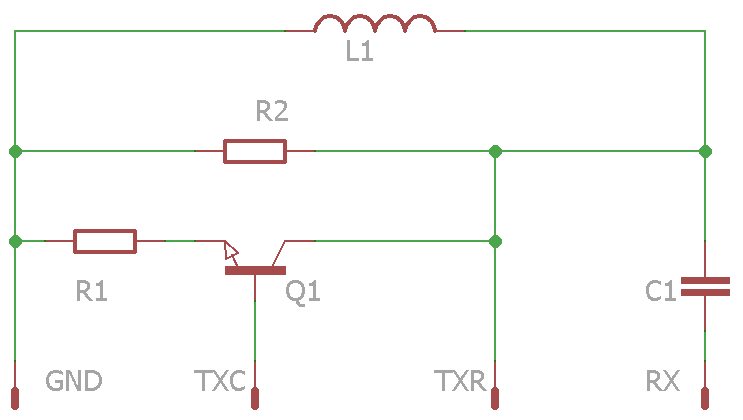
\includegraphics[width=\linewidth]{img/antennaschematic}
  \caption{Antenna Schematic}
  \label{fig:antennaschematic}
\end{figure}

\begin{figure}[h]
  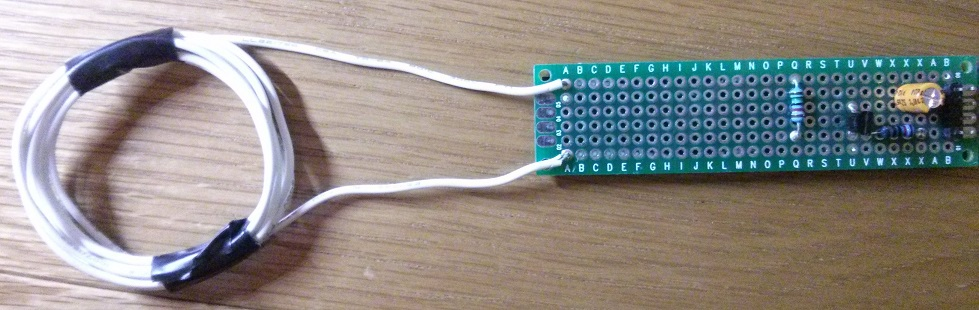
\includegraphics[width=\linewidth]{img/antennapic}
  \caption{Antenna PCB}
  \label{fig:antennapic}
\end{figure}


Though we discuss the antenna more in Section \ref{sec:evaluation}, we mention here that the range for eavesdropping on both reader and tag (which is further away) was only about 1-2 cm. To remedy this, we taped the antenna to the back of the RC522 reader, and the tag to be read to the front of it as shown in Figure \ref{fig:setup}. The picture taken is before the final PCB was made, and with a different NFC tag (still using the NTAG203 chip).


\begin{figure}[h]
  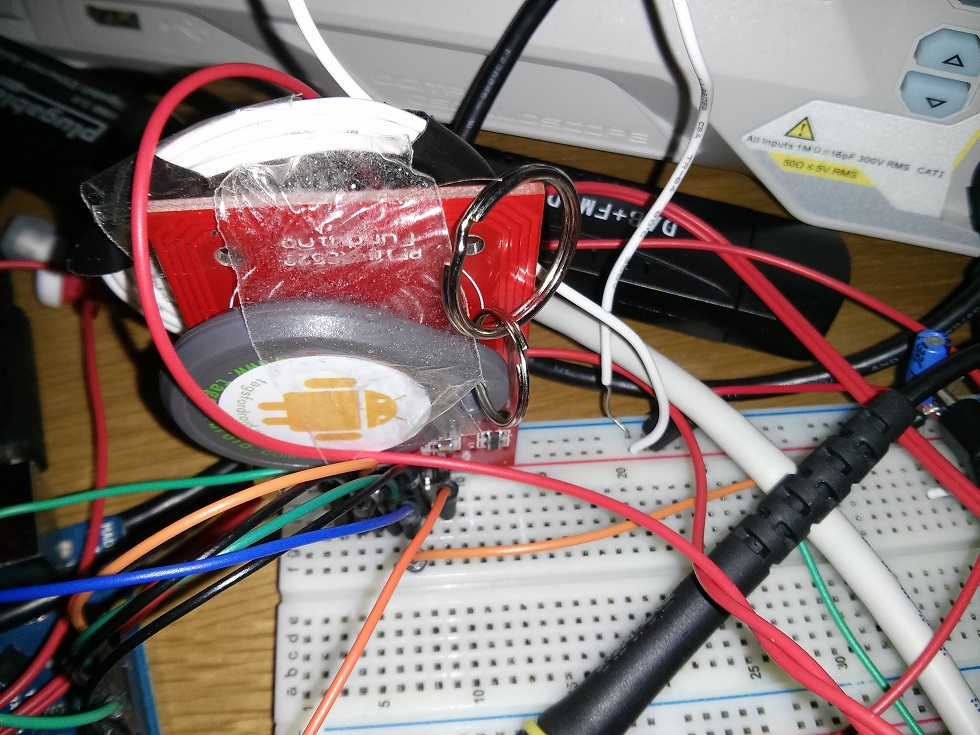
\includegraphics[width=\linewidth]{img/setup}
  \caption{Measurement Setup}
  \label{fig:setup}
\end{figure}


%%%% FOR NEXT SECTION
\begin{figure*}[!t]
  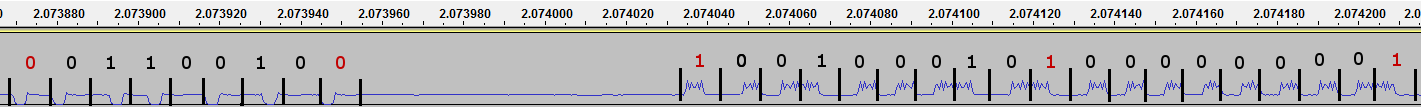
\includegraphics[width=\textwidth]{img/annotated}
  \caption{Annotated Recoding}
  \label{fig:annotated}
\end{figure*}

\subsection{Eavesdropping}
\label{subsec:eavesdrop}

For consistency/determinism, and easy testing/reproducibility, we initially recorded the interaction between the reader and the tag. This was achieved by using our home-made antenna connected to the USRP in the setup shown in Figure \ref{fig:setup}. The {\em envelope} of the signal is sufficient for our purposes, and for our Amplitude Modulated (AM) signal can be calculated as the absolute value of the signal. Recoding the envelope as a WAV file (using GNU Radio's \texttt{wavfile\_sink}) using a sample rate of $2,000,000$ samples/second and a 16-bit output, we get around 4 MB of data to be processed per second.

Opening the resulting audio file in Audacity Audio Editor, we see that for PCD transmissions the signal drops close to 0, while for PICC transmissions the subcarrier spikes hover at about 5-10\% above the average. An annotated example of the REQA and ATQA transmissions is shown in Figure \ref{fig:annotated}, where start/end and parity bits are shown in red. 


Consequently, we can detect such transitions by having a moving window (say of length $2,000$) that keeps track of the average, and if the next value is below a certain threshold ($10\%$ of the average), consider it part of a reader transmission, and if it goes above a different threshold ($110\%$ of the average), consider it part of a card transmission. The transmission is considered over when the signal has returned to its average values for too long (currently $>25\ms$), and to ensure that the average does not drift, values above the high threshold and below the low threshold are not included in the moving average. The duration and values of these transitions are then passed on to the appropriate decoders through callbacks, so that the decoding runs in a background thread.

The two decoders (one for Manchester encoding, and the other for the Modified Miller Encoding) are essentially Finite State Machines (FSM) that implement the specifications mentioned in Sections \ref{subsec:pcd} and \ref{subsec:picc}, allowing for some margin of transmission and measurement errors. For instance, the sequence $[(0, 3), (1, 11), (0, 3), (1, 16), (0, 3), (1, 6)]$ of (bit, \ms duration) pairs would be (approximately) split as:

\begin{align}
\nonumber [(0, 3), (1, 6.5)] \rightarrow& 0&\\
\nonumber [(4.5, 1), (0, 3), (1, 1.5)]\rightarrow & 1&\\
\nonumber [(1, 9.5)] \rightarrow & 0 &\\
\nonumber [(1, 5), (0, 3), (1, 1.5)] \rightarrow & 1 &\\
\nonumber  (1, 4.5) \rightarrow & \text{state=ONE\_FIRST\_STAGE} &
\end{align}

Having recovered all the bits (including parity, but discarding any start/end bits), and knowing whether the PCD or the PICC is doing the transmission, these bits can be interpreted with context in a more high-level FSM. This is the code that updates the internal state of the tag/reader when needed (e.g. to decrypt bits in the MIFARE Classic case), ensures that the parity is correct and transforms bits into bytes, and then based on the current state and the ``header" of the incoming bytes determines the command issued, interprets the bytes and checks any CRC if necessary. 

For unencrypted commands, this process is not crucial,\footnote{Indeed, the code will just print the plaintext bytes in case it cannot interpret them.} but for the Classic 1K, parsing the commands to get the UID, for instance, is of utmost importance as any deviations would result in ciphertext that cannot by decrypted. Specifically for regular data transmission decryption is straightforward, but the setup phase of the challenge-response protocol needs to be handled more subtly, especially because of nested authentications after the first authentication. Hence, while the actual cipher is abstracted away into a different class, it is the responsibility of the FSM to correctly call it.

\subsection{Emulating}
\label{subsec:emulate}

The FSM proved to be an important abstraction for the emulation part of the project because it centralized also encryption considerations. As a result, the emulated Reader and Tag only deal with plaintext messages (and not individual bits). Specifically, the Reader is set to perform identically to the Arduino's DumpInfo program, by performing the anticollision, and then reading all card blocks. The Tag is programmed to respond to the incoming commands, and its memory layout is set dynamically through files. For reproducibility (and especially when emulating the tag against a recording), the randomness used by the Tag and the Reader can also be fixed, but they can also be generated on-the-fly as needed, ensuring that this is not merely a replay attack.

Because of this setup, it is possible to emulate both the reader and the tag simultaneously, without needing to go through encoding and modulation, but we have also coded the Manchester and Modified Miller encodings (in a reverse fashion to Section \ref{subsec:eavesdrop}), as well as modulation, which can be output to a WAV file for use without a USRP.

Modulating the Reader's output is straightforward: it is enough to generate a 13.56 MHz (sine wave) carrier and output it, or output nothing for the ``pause" duration. Load Modulation of the Tag is more complicated, and is achieved by only outputting when the encoding is a logical 1 (for either 4.5\ms or 9\ms). Specifically, however, and as explained in Section \ref{subsec:picc} (Figure \ref{fig:manchester}), this is achieved by generating a 847.5 kHz subcarrier, multiplying by the bit to output, and the switching the load (in this case through the transistor) only for the amount of time for which the signal is positive.

%----------------------------------------------------------------------------------------
%	EVALUATION
%----------------------------------------------------------------------------------------


%%%%  FOR NEXT SECTION
\begin{figure*}[ht]
  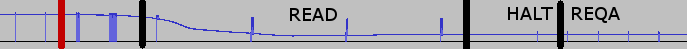
\includegraphics[width=\linewidth]{img/usrpreal}
  \caption{Signal Received when Approaching Tag}
  \label{fig:usrpreal}
\end{figure*}


\begin{figure*}[ht]
  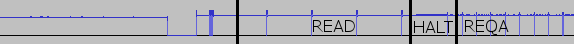
\includegraphics[width=\linewidth]{img/usrpreset}
  \caption{Signal Received with Fixed Tag and Arduino Reset}
  \label{fig:usrpreset}
\end{figure*}


\section{Evaluation}
\label{sec:evaluation}

explain

\subsection{Eavesdropping}

First of all, it is worth mentioning that with recorded reader-tag communications, the eavesdropping code behaves predictably and always correctly decodes the messages. However, at least initially the code required 50 seconds of processing per 1 second of data. This was due to the fact that incoming messages in GNU Radio Python code are stored as \texttt{NumPy} arrays which do not support efficient iteration. Converting them to a list before iteration resulted in a $10\times$ improvement, and assigning local names to function calls resulted in an additional $2.5\times$ improvement, for a processing cost of about 2.2 seconds per 1 second of data.

This is still not real time, but given the unusual setup which relies heavily on the USB bus, this performance is acceptable given the convenience Python presents for prototyping. That said, the setup could have substantially benefited from a more fine-tuned antenna. As mentioned in Section \ref{subsec:antenna}, the range was only a couple of centimeters, and this was certainly not improved by the lack of a proper connecting cable and shielding. 

In the Do-It-Yourself (DIY) spirit, we also attempted to create an amplifier (which unfortunately would not be a Low-Noise Amplifier) based on the design in \cite{amplifier} with a couple of minor resistance modifications to make it work with 9V. However, the modifications did no quite work, but instead resulted in signal distortion as shown in Figure \ref{fig:amplified}.

\begin{figure}[h]
  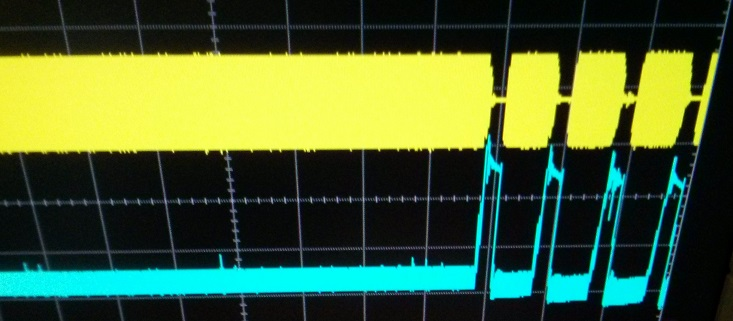
\includegraphics[width=\linewidth]{img/amplified}
  \caption{Failed Amplification: Original in Yellow and ``Amplified" in Blue}
  \label{fig:amplified}
\end{figure}

This setback thus necessitated the setup shown in Figure \ref{fig:setup} where the PCD, the PICC, and our antenna are in close proximity. However, we also tested a more ``real-world" situation, where the user approaches the reader with the tag. This is shown in Figure \ref{fig:usrpreal}, where the signal strength drops when the tag starts approaching reader (due to their coupling --- indicated by red). As can be seen, the signal strength is not sufficient to recover the tag's transmission during the anticollision and selection phases, but it is can recover them after the first READ request. This would be insufficient for MIFARE Classic cards, but it does result in partial recovery for the Ultralight card.

It is worth pointing out that the Reader commands are fully decoded even during the signal strength changes. This is remains true and is even more pronounced in Figure \ref{fig:usrpreset}, where the Arduino is reset (but the tag remains close to the reader). The moving average methodology, then, works well, and we have included a couple of example traces received in Appendix \ref{app:traces} for reference and completeness.

\subsection{Emulating}

There is not much to say about software emulation (either of both reader and tag, or of one of them against a recorded WAV file), except that it works, but does not adhere to the ISO and MIFARE timing requirements. Specifically, due to the fact that the signal processing is not real-time, it did not seem prudent to focus on clock recovery/synchronization and implementing timeouts, as it would be impossible to test them within the confines of our system.


\begin{figure}[h]
\centering
\begin{minipage}[b]{.47\linewidth}
  \centering
  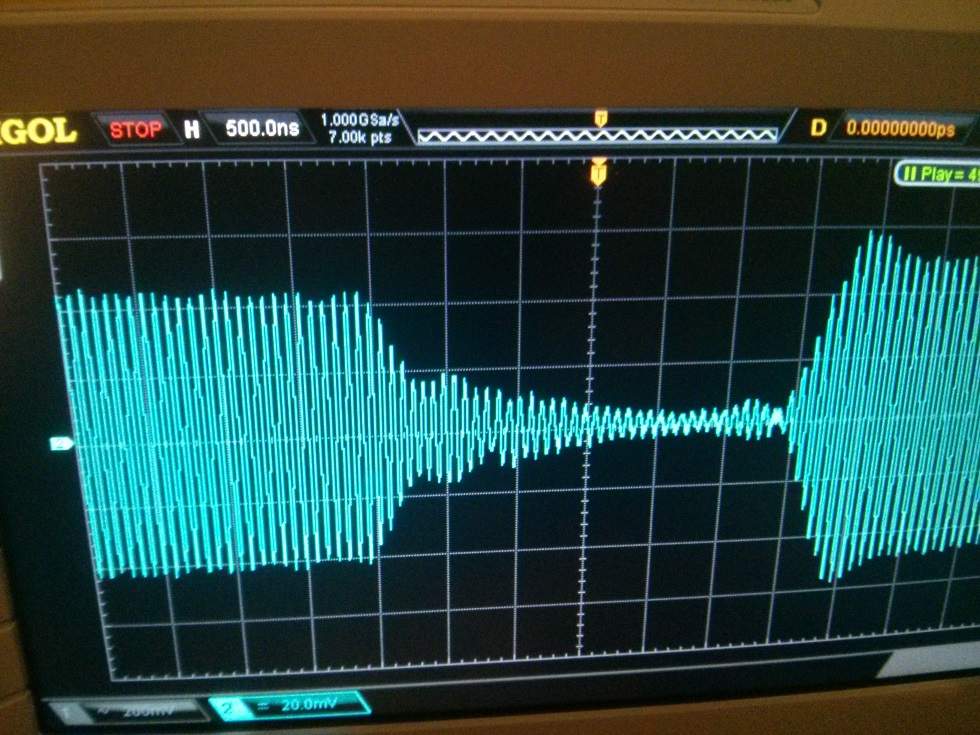
\includegraphics[width=\textwidth]{img/emulated}
  \captionof{figure}{Emulated Signal}
  \label{fig:emulated}
\end{minipage}
\begin{minipage}[b]{.47\linewidth}
  \centering
  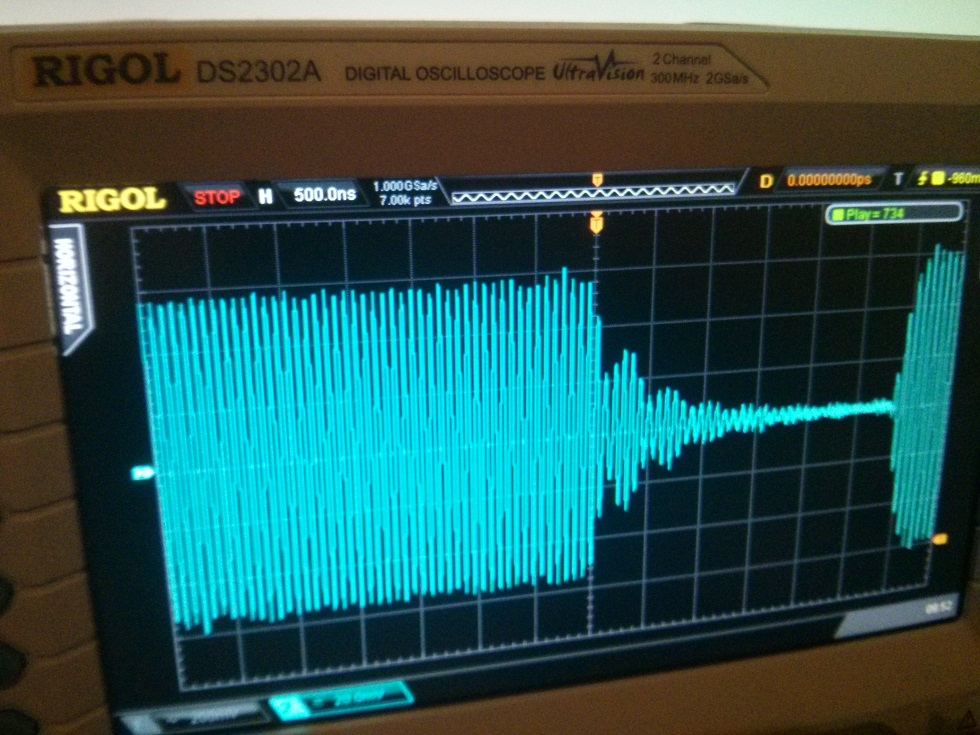
\includegraphics[width=\textwidth]{img/real}
  \captionof{figure}{Real Signal}
  \label{fig:real}
\end{minipage}
\end{figure}

However, this makes it harder to test the transmissions against real hardware. Testing the reader emulation is somewhat easier because the reader generate its own carrier. Specifically, as shown in Figure \ref{fig:emulated}, the emulated signal closely resembles the signal of a real reader (Figure \ref{fig:real}). Moreover, as shown in figure \ref{fig:readertx}, we see in yellow that the USRP signal sent is not particularly strong, and the reception on the (unpowered) RC522 reader antenna in blue already indicates a strength drop due to our untuned transmissions.


\begin{figure}[h]
  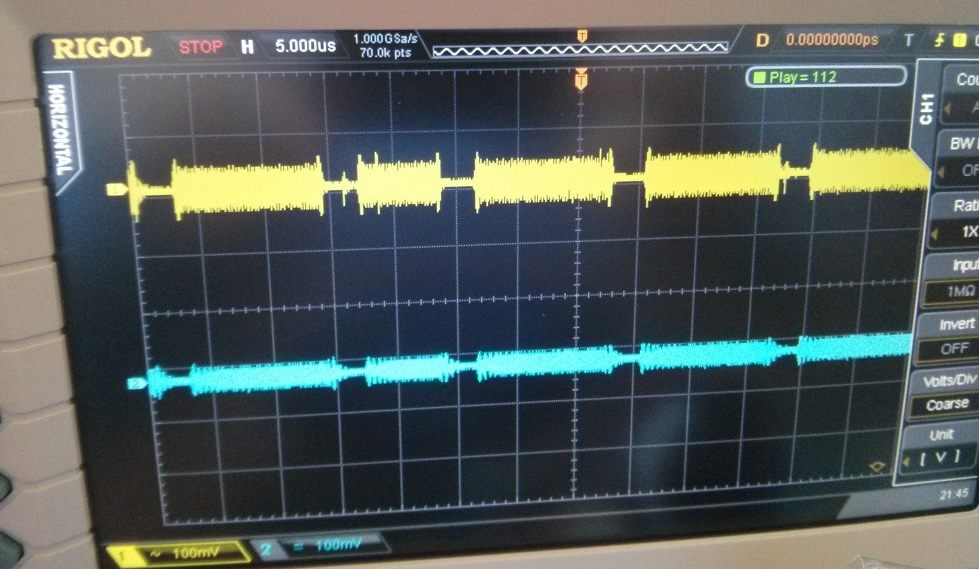
\includegraphics[width=\linewidth]{img/readertx}
  \caption{Reader TX in Yellow, RC522 Antenna in Blue}
  \label{fig:readertx}
\end{figure}


The implementation of the hardware tag emulation was not as successful. Specifically, even with the LFTX daughterboard, we could not get any signal transmission out of the USRP at the 847.5 kHz range, so we had to up the frequency to 13.56 MHz. The behavior of the signal strength is similar to the Reader TX (Figure \ref{fig:tagtx}), but because of the lack of synchronization, this means that when the RC522 Reader is on, the signals overlap, as shown in Figure \ref{fig:overlap}. We used this to our advantage and confirmed that it could be used for (dynamic) interference in response to data being sent (although with some processing lag), since on the Arduino end, this lead to timeouts and other errors.


\begin{figure}[h]
  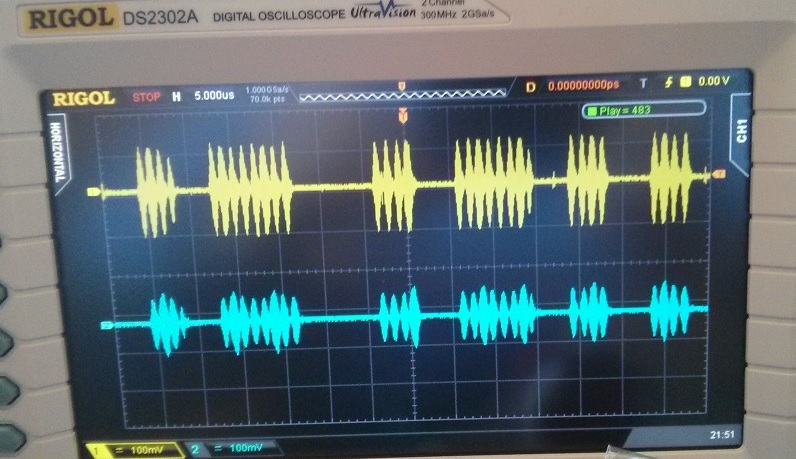
\includegraphics[width=\linewidth]{img/tagtx}
  \caption{Tag TX in Yellow, RC522 Antenna in Blue}
  \label{fig:tagtx}
\end{figure}


\begin{figure}[h]
  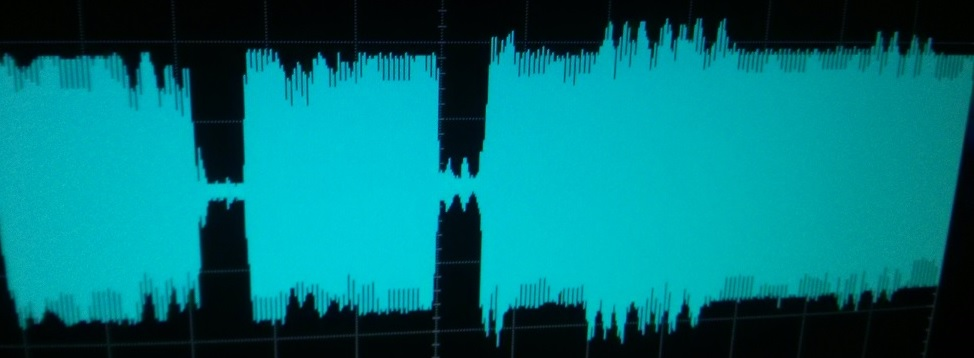
\includegraphics[width=\linewidth]{img/overlap}
  \caption{Tag TX Overlap with RC522 Reader}
  \label{fig:overlap}
\end{figure}

??? what is output like?

%----------------------------------------------------------------------------------------
%	CONCLUSIONS
%----------------------------------------------------------------------------------------

\section{Conclusions}
\label{sec:conclusions}
and future work

lack of newer cards eg desfire and ultralight ev

need better setup (laptop-wise)
better antenna

makes sense why coding in FPGA/C,  but sufficient even under bad setup

ideal if had embedded solutions in hand

should really do clock sync, but would need to re-work architecture


%----------------------------------------------------------------------------------------
%	ACKNOWLEDGMENTS
%----------------------------------------------------------------------------------------

\phantomsection
\section*{Acknowledgments} % The \section*{} command stops section numbering

I would like to thank Kasper Rasmussen for being my supervisor, for his invaluable help throughout the project, and for entrusting me with his expensive equipment. I would also like to thank Simon Crowe for helping shape the focus of the project. Finally, I would like to thank Kellogg College and their Research Support Grant which enabled the purchase of some of the components that were used in this project.

%----------------------------------------------------------------------------------------
%	BIBLIOGRAPHY
%----------------------------------------------------------------------------------------
\phantomsection
\bibliographystyle{acm}
\bibliography{bibliography}

%----------------------------------------------------------------------------------------
%	APPENDIX
%----------------------------------------------------------------------------------------

\onecolumn
\appendix

\phantomsection
\section*{Appendices}
\addcontentsline{toc}{section}{Appendices}
\renewcommand{\thesubsection}{\Alph{subsection}}

\subsection{MIFARE Cards}
\label{app:mifare}
In this section, we focus on the MIFARE Ultralight and Classic 1K cards, with more general ISO details in \cite{iso144433}.

\subsubsection{MIFARE Ultralight \cite{ultralight}}
\label{app:ultralight}

The memory layout for a MIFARE Ultralight card can be found in Figure \ref{fig:memul}. The card has a 7-byte UID SN[0-6], including 2 check bytes BCC[0-1]. SN0 is the manufacturer ID (0x04 for NXP Semiconductors), and the check bytes are defined as follows: $BCC0=0x88 \oplus SN0 \oplus SN1 \oplus SN2$ and $BCC1 = SN3 \oplus SN4 \oplus SN5 \oplus SN6$. Lock bytes can be used to turn pages into read-only mode, while One-Time Pad (OTP) bytes can be set to 1, but never set back to 0 again. As can be seen in Figure \ref{fig:fsmul}, Ultralight cards go through 2 rounds of ANTICOLLISION and SELECT commands.


\begin{figure}[h]
\centering
\begin{minipage}[b]{.47\textwidth}
  \centering
  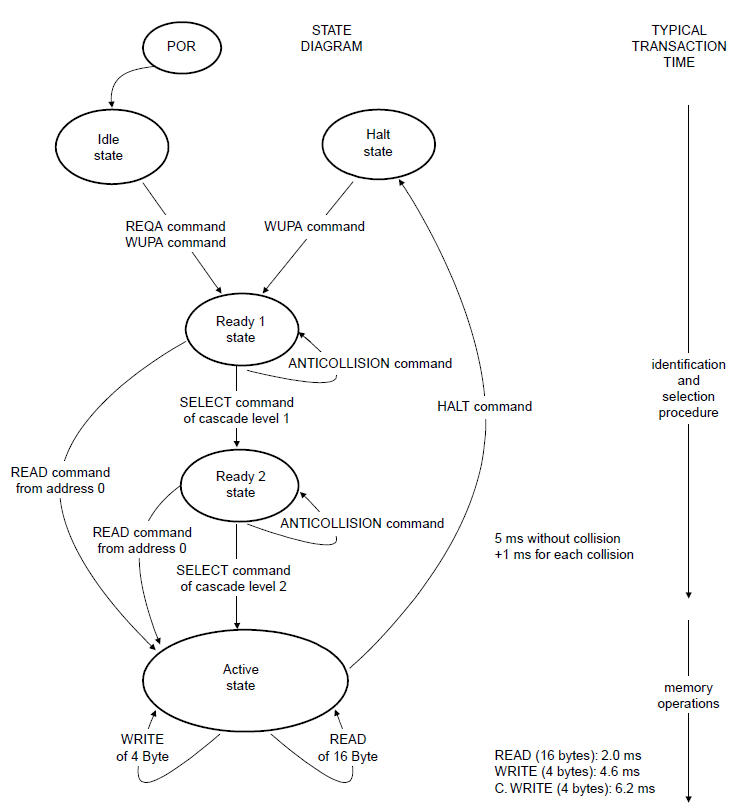
\includegraphics[width=\textwidth]{img/fsmul}
  \captionof{figure}{MIFARE Ultralight FSM}
  \label{fig:fsmul}
\end{minipage}
\begin{minipage}[b]{.47\textwidth}
  \centering
  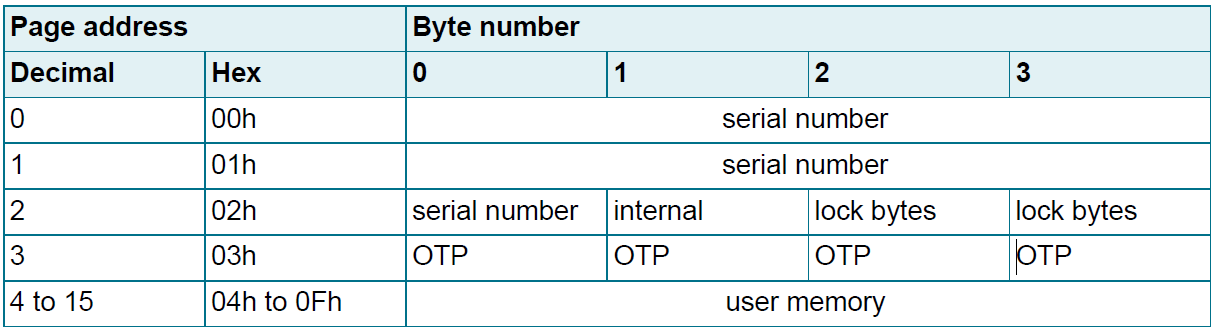
\includegraphics[width=\textwidth]{img/memul}
  \captionof{figure}{MIFARE Ultralight Memory Layout}
  \label{fig:memul}
\end{minipage}
\end{figure}

\noindent Table \ref{tab:cmdul} shows the possible commands when communicating with a MIFARE Ultralight card. The address for the READ and WRITE commands are between 0x00 and 0x0F and include roll-over  C[0-1] is the CRC, and D[0-15] refers to data bytes.

\begin{table}[h]
\centering
\caption{MIFARE Ultralight Commands}
\label{tab:cmdul}
\begin{tabular}{|l|l|l|}
\hline
\rowcolor{headcolor}
{\bf Command} 		&     {\bf Code} 						&    {\bf Response} 		\\ \hline
REQA 				&     0x26      						&    0x44  0x00 (ATQA) 		\\ \hline
WUPA 			&     0x52      						&    0x44  0x00 (ATQA) 		\\ \hline
ANTICOLLISION (1)  	&     0x93 0x[20-67]     					&    0x88 SN0 SN1 SN2 BCC0       	\\ \hline
SELECT (1) 			&     0x93 0x70 0x88 SN0 SN1 SN2 BCC0 C0 C1       	&    0x04 C0 C1			\\ \hline
ANTICOLLISION (2)		&     0x95 0x[20-67]				       	&    SN3 SN4 SN5 SN6 BCC1        	\\ \hline
SELECT (2) 			&     0x95 0x70 SN3 SN4 SN5 SN6 BCC1 C0 C1       	&    0x00 C0 C1			\\ \hline
READ 				&     0x30 [Addr] C0 C1					&    D0 D1 $\cdots$ D15 C0 C1    	\\ \hline
WRITE 			&     0xA2 [Addr] D0 D1 D2 D3 C0 C1       		&   [ACK/NAK]		         	\\ \hline
COMPATIBILITY WRITE (1)&     0xA0 [Addr] C0 C1 					&   [ACK/NAK]			\\ \hline
COMPATIBILITY WRITE (2)&     D0 D1 $\cdots$ D15 C0 C1				&   [ACK/NAK]			\\ \hline
HALT				&     0x50 0x00 C0 C1				       	&   [passive ACK/NAK]             	\\ \hline
\end{tabular}
\end{table}

\newpage
\subsubsection{MIFARE Classic 1K \cite{classic1k}}
\label{app:classic1k}

The memory layout for Classic 1K cards can be seen in Figure \ref{fig:mem1k}. The card does not have a globally-unique identifier, but instead uses a 4-byte Non-Unique Identifier (NUID) in block 0. Each sector has a block called the ``trailer", which contains the two keys and the access bits. The layout for these access bits is shown in Figure \ref{fig:access}, where $CX_y$ is the $X$'th access bit for block $y$. These access bits are interpreted differently based on whether the block is a trailer block (Figure \ref{fig:trailer}) or a data block (Figure \ref{fig:data}).

\begin{figure}[h]
\centering
\begin{minipage}[b]{.47\textwidth}
  \centering
  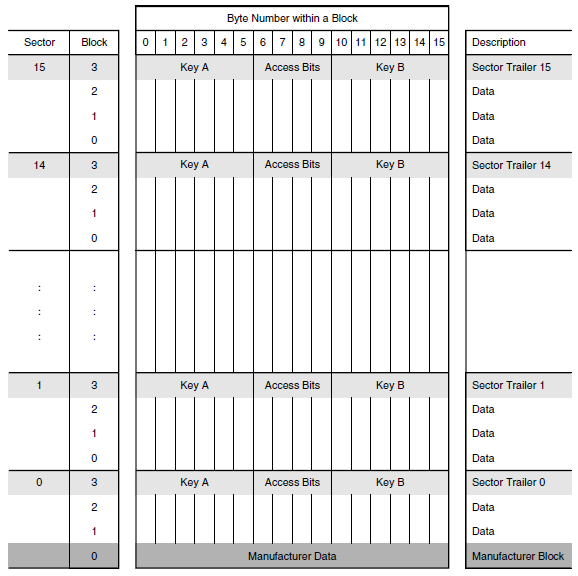
\includegraphics[width=\textwidth]{img/mem1k}
  \captionof{figure}{MIFARE Classic 1K Memory Layout}
  \label{fig:mem1k}
\end{minipage}
\begin{minipage}[b]{.47\textwidth}
  \centering
  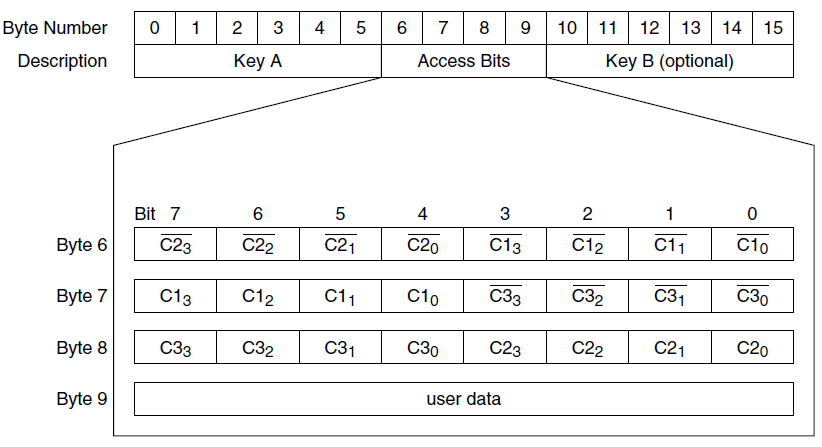
\includegraphics[width=\textwidth]{img/access}
  \captionof{figure}{MIFARE Classic 1K Access Bits}
  \label{fig:access}
\end{minipage}
\end{figure}



\begin{figure}[h]
\centering
\begin{minipage}[b]{.47\textwidth}
  \centering
  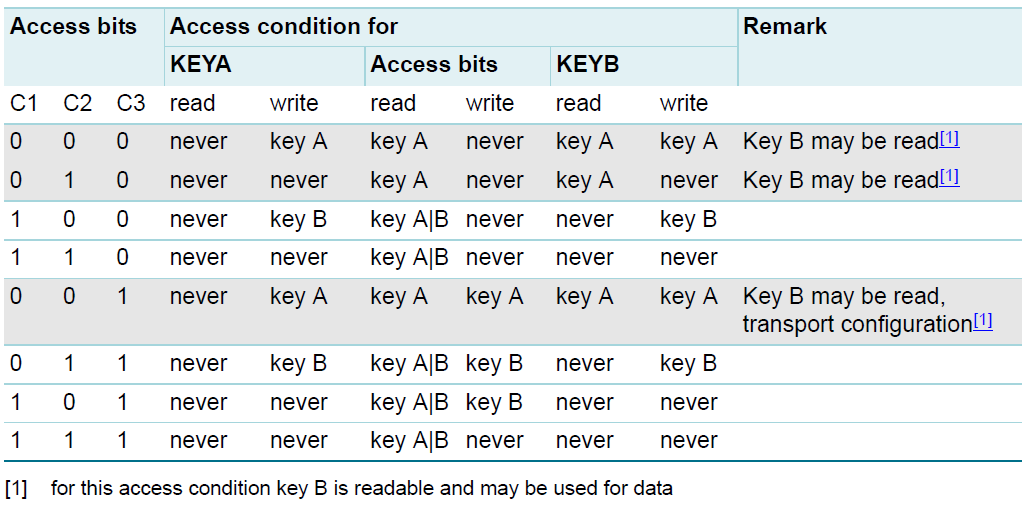
\includegraphics[width=\textwidth]{img/trailer}
  \captionof{figure}{Trailer Block Access Conditions}
  \label{fig:trailer}
\end{minipage}
\begin{minipage}[b]{.47\textwidth}
  \centering
  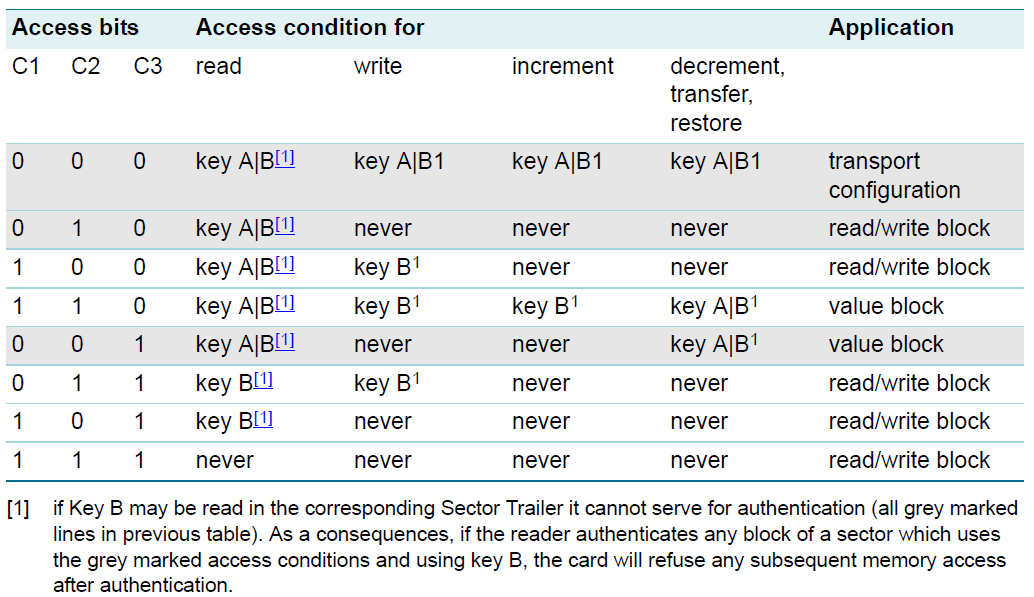
\includegraphics[width=\textwidth]{img/data}
  \captionof{figure}{Data Block Access Conditions}
  \label{fig:data}
\end{minipage}
\end{figure}

It is worth noting that the data blocks can be used for simple read/write operations, or they can be used as ``value blocks" for applications which need more robustness and backups and could benefit from operations like INCREMENT and DECREMENT (see below). The layout for such blocks is shown in Figure \ref{fig:value}.

\begin{figure}[h]
  \hfill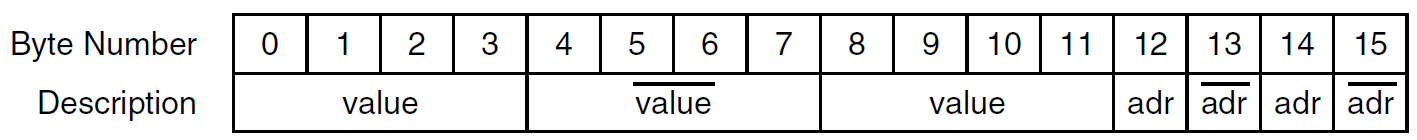
\includegraphics[width=0.7\linewidth]{img/value} \hspace*{\fill}
  \caption{Value Block Layout}
  \label{fig:value}
\end{figure}

\noindent As indicated in Figure \ref{fig:fsm1k}, the Classic 1K only uses a single round of ANTICOLLISION and SELECT commands, but includes a much more complicated 3-pass authentication mechanism. We explain in detail the encryption scheme in Appendix \ref{app:crypto1}, but we include the un-encrypted commands in Table \ref{tab:cmd1k}, where NID[0-3] represents the NUID and $BCC=NID0 \oplus NID1 \oplus NID2 \oplus NID3$. Addresses range from 0x00 to 0x3F, while C[0-1] refers to the Checksum and D[0-15] to data bytes.

\begin{figure}[ht]
 \hfill
  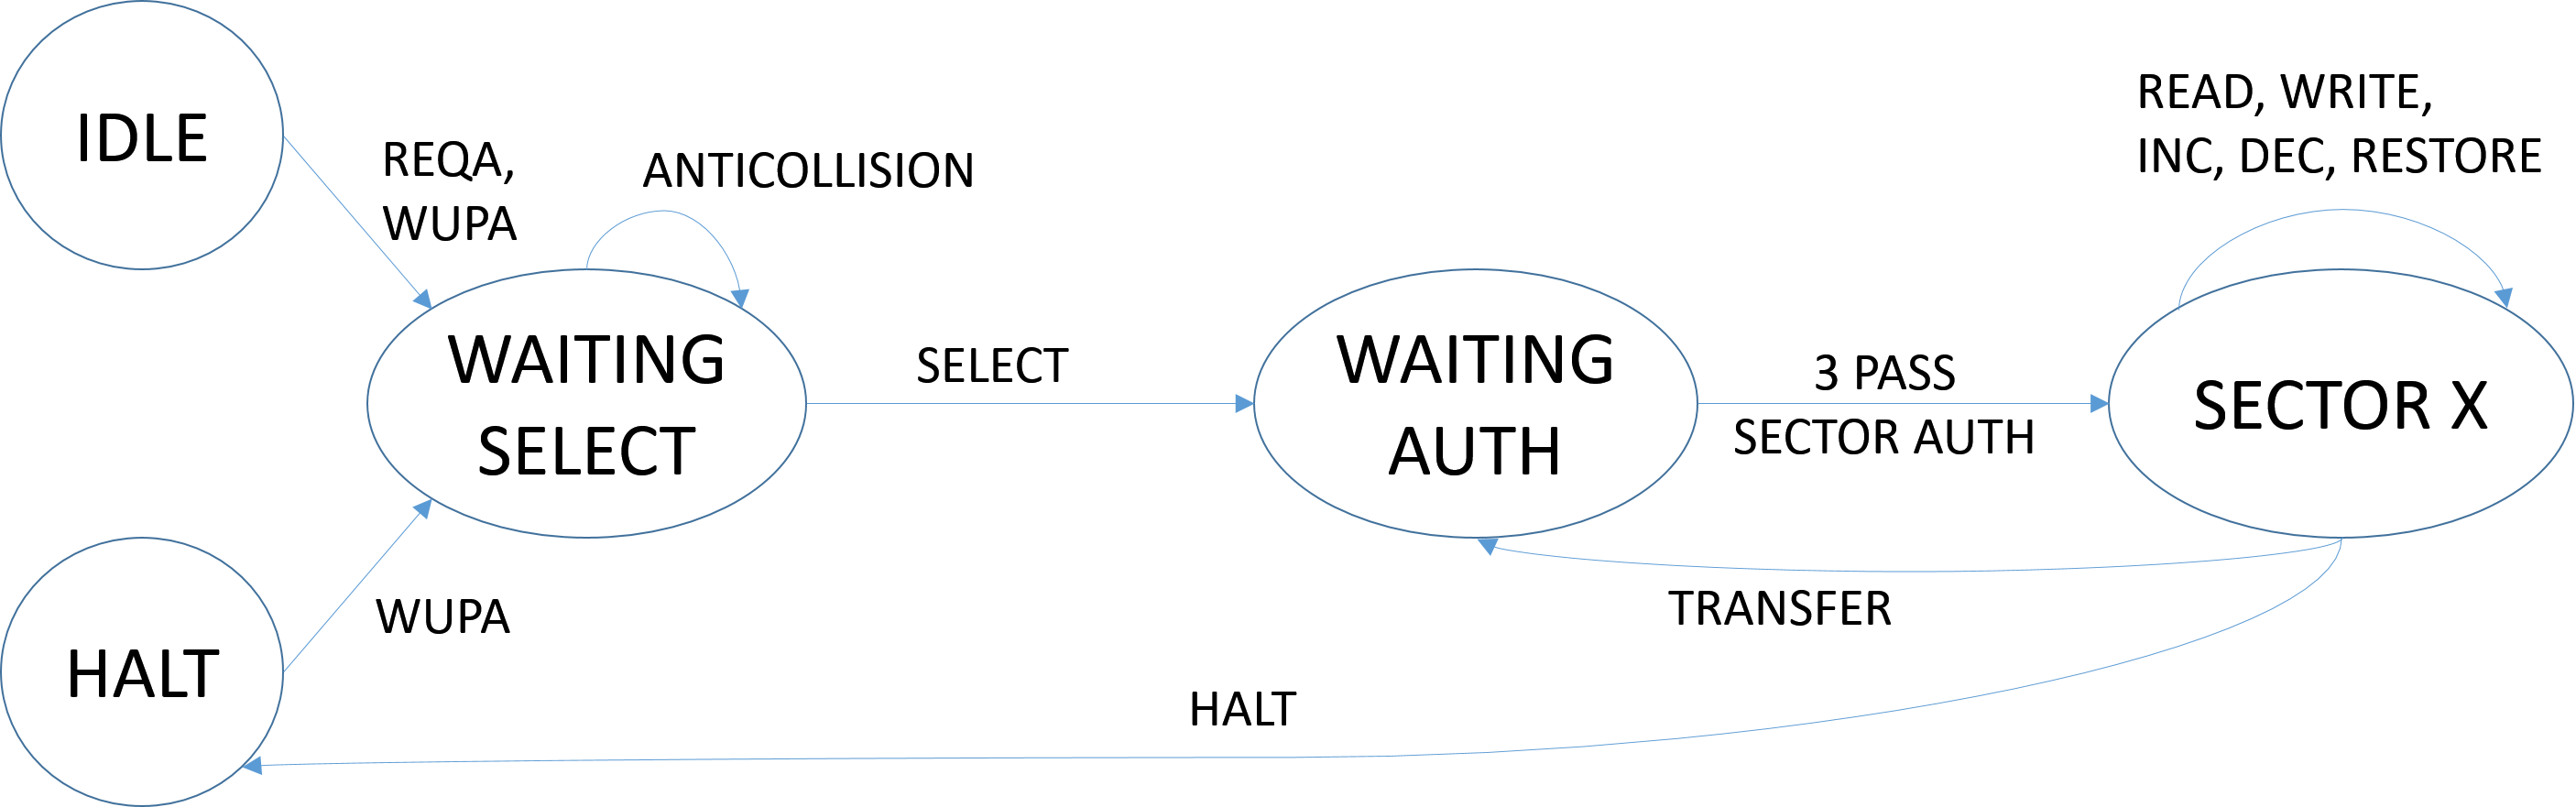
\includegraphics[height=7cm,keepaspectratio]{img/fsm1k}
 \hspace*{\fill}
  \caption{Classic 1K FSM}
  \label{fig:fsm1k}
\end{figure}



\begin{table}[ht]
\centering
\caption{MIFARE Classic 1K Plaintext Commands}
\label{tab:cmd1k}
\begin{tabular}{|l|l|l|}
\hline
\rowcolor[HTML]{E2F1F3} 
{\bf Command} 		&     {\bf Code} 						&    {\bf Response} 		\\ \hline
REQA 				&     0x26      						&    0x04  0x00 (ATQA) 		\\ \hline
WUPA 			&     0x52      						&    0x04  0x00 (ATQA) 		\\ \hline
ANTICOLLISION	  	&     0x93 0x20     						&    NID0 NID1 NID2 NID3 BCC   	\\ \hline
SELECT  			&     0x93 0x70  NID0 NID1 NID2 NID3 BCC C0 C1  	&    0x08 C0 C1			\\ \hline
AUTHA			&     0x60 [Addr] C0 C1					&    D0 D1 D2 D3  [TOKEN RB]    	\\ \hline
AUTHB			&     0x61 [Addr] C0 C1					&    D0 D1 D2 D3  [TOKEN RB]	\\ \hline
AUTH3 [TOKEN AB]		&     D0 D1 $\cdots$ D7					&    D0 D1 D2 D3  [TOKEN BA]	\\ \hline
READ 				&     0x30 [Addr] C0 C1					&    D0 D1 $\cdots$ D15 C0 C1    	\\ \hline
WRITE (1)			&     0xA0 [Addr] C0 C1 					&   [ACK/NAK]			\\ \hline
WRITE (2)			&     D0 D1 $\cdots$ D15 C0 C1				&   [ACK/NAK]			\\ \hline
INCREMENT (1)		&     0xC1 [Addr] C0 C1					&   [ACK/NAK]			\\ \hline
DECREMENT (1)		&     0xC0 [Addr] C0 C1					&   [ACK/NAK]			\\ \hline
RESTORE (1)			&     0xC2 [Addr] C0 C1					&   [ACK/NAK]			\\ \hline
INC/DEC/RES (2)		&     D0 D1 $\cdots$ D15 C0 C1				&   [passive ACK/NAK]		\\ \hline
TRANSFER			&     0xB0 [Addr] C0 C1					&   [ACK/NAK]			\\ \hline
HALT				&     0x50 0x00 C0 C1				       	&   [passive ACK/NAK]             	\\ \hline
\end{tabular}
\end{table}

\newpage
\subsection{CRYPTO1}
\label{app:crypto1}

In this section, we summarize the CRYPTO1 algorithm as reverse-engineered in \cite{crypto1, classicvulnerabilities}, but do not discuss the numerous vulnerabilities with the cipher which are addressed in the original papers. In the notation of \cite{classicvulnerabilities}, let the (unencrypted) nonce RB be denoted by $n_T$, the token AB be denoted as $\{n_R\},\{a_R\}$ and the token BA be denoted as $\{a_T\}$. Also denote by $k$ the key, $u$ the tag's unique identifier (UID), and for any $x$, let $x_i$ be its $i$-th bit (for $i$ for which this is well-defined). The CRYPTO1 algorithm uses a Linear Feedback Shift Register (LFSR) of size equal to 48 bits which is initialized by the key (also of length 48). Thus, as $\alpha_i=a_i a_{i+1}\ldots a_{i+47}$ the internal state of the LFSR at time $i$, we get that:

\begin{itemize}[nosep]
\item $a_i := k_i$, for $0\le i \le 47$
\item $a_{48+i} := L(a_i,\ldots,a_{47+i}) \oplus n_{T,i} \oplus u_i$, for $0 \le i \le 31$
\item $a_{80+i} := L(a_{32+i},\ldots,a_{79+i}) \oplus n_{R,i}$, for $0 \le i \le 31$
\item $a_{112+i} := L(a_{64+i},\ldots,a_{111+i})$, $\forall i \in \mathbb{N}$
\end{itemize}
where $L$ is the LFSR ``{\bf feedback function}" defined by:

\noindent $L(x_0x_1\ldots x_{47}):=x_{0} \oplus x_{5} \oplus x_{9} \oplus x_{10} \oplus x_{12} \oplus x_{14} \oplus x_{15} \oplus x_{17} \oplus x_{19} \oplus x_{24} \oplus x_{25} \oplus x_{27} \oplus x_{29} \oplus x_{35} \oplus x_{39} \oplus x_{41} \oplus x_{42} \oplus x_{43}$


The outputs are encrypted using a ``{\bf filter function}":

\noindent $f(x_0x_1\ldots x_{47}) := f_c(f_a(x_9,x_{11},x_{13},x_{15}),f_b(x_{17},x_{19},x_{21},x_{23}),f_b(x_{25},x_{27},x_{29},x_{31}),f_a(x_{33},x_{35},x_{37},x_{39}),f_b(x_{41},x_{43},x_{45},x_{47}))$, where 
\begin{align}
\nonumber f_a(y_0,y_1,y_2,y_3):=&((y_0 \vee y_1) \oplus (y_0 \wedge y_3)) \oplus (y_2 \wedge ((y_0 \oplus y_1) \vee y_3)) &\\
\nonumber f_b(y_0,y_1,y_2,y_3):=&((y_0\wedge y_1) \vee y_2) \oplus ((y_o \oplus y_1) \wedge (y_2 \vee y_3)) &\\
\nonumber f_c(y_0,y_1,y_2,y_3,y_4):=&(y_0 \vee ((y_1 \vee y_4) \wedge (y_3 \oplus y_4))) \oplus ((y_0 \oplus (y_1 \wedge y_3)) \wedge ((y_2 \oplus y_3) \vee (y_1 \wedge y_4))) &
\end{align}

These two main functions are summarized in Figure \ref{fig:lfsr}.

\begin{figure}[h]
  \hfill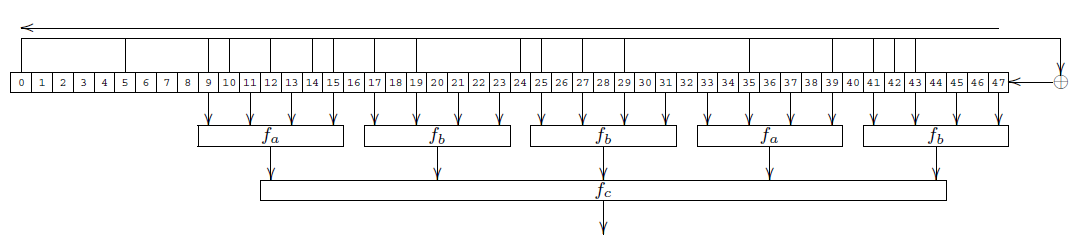
\includegraphics[width=\linewidth]{img/lfsr} \hspace*{\fill}
  \caption{Crypto1 LFSR \cite{classicvulnerabilities}}
  \label{fig:lfsr}
\end{figure}

The keystream bit $b_i$ is then defined by $b_i := f(a_i\ldots a_{47+i})$, and the encryptions of the $i$-th regular bit (i.e. excluding start/end and parity bits) is defined by XORing with $b_i$. Specifically, for $0\le i \le 31$, $\{n_{R,i}\}=n_{R,i} \oplus b_{32+i}$, $\{a_{R,i}\}=a_{R,i} \oplus b_{64+i}$, $\{a_{T,i}\}=a_{T,i} \oplus b_{96+i}$. Note that the first 32 bits are not used in the first authentication, but they are used in all subsequent authentications, as the tag nonce is encrypted (and the cipher is re-initialized), so that $\{n_{T,i}\}=n_{T,i} \oplus b_i$. 

The challenges only depend on the random nonce $n_T$, with $a_R=suc^{64}(n_T)$ and $a_T=suc^{96}(n_T)$, where the ``{\bf successor function}" (used for the Pseudo Random Number Generation (PRNG) is iteratively applied 64 and 96 times respectively. It is defined by $suc(x_0x_1\ldots x_{31}):=x_1x_2\ldots x_{31}(x_{16}\oplus x_{18}\oplus x_{19}\oplus x_{21}))$ which only depends on the last 16 bits of the input.


It is worth noting that the start and ending transmission bits are not encrypted, but the parity bits are --- by reusing the encryption bit for the next bit to be encrypted: $\{p_j\} :=p_j \oplus b_{8j +8}$. This leaks information, and makes the protocol incompatible with the ISO standard, since the parity bits can be inverted. See Appendix \ref{app:traces} for an example.


\subsection{Example Traces}
\label{app:traces}

In this section we show two example traces, one for the MIFARE Ultralight (Table \ref{tab:traceul}) and one for the Classic 1K (Table \ref{tab:trace1k}). For the latter, only part of the trace is shown. The key used is 0xFF 0xFF 0xFF 0xFF 0xFF 0xFF, and the exclamation points indicate inverted parity bits.

\begin{center}
\begin{longtable}{|l|l|l|}
\caption{MIFARE Ultralight Trace}\label{tab:traceul}\\   
\hline
\rowcolor{headcolor}
{\bf Direction} 		&     {\bf Bytes} 						&    {\bf Explanation} 	\\ \hline
PCD$\rightarrow$PICC 	& 0x26							&    REQA			\\ \hline
PICC$\rightarrow$PCD 	& 0x44 0x00							&    ATQA			\\ \hline


PCD$\rightarrow$PICC 	& 0x93 0x20							&    ANTICOLLISION (1)	\\ \hline
PICC$\rightarrow$PCD 	& 0x88 0x04 0xBE 0x6F 0x5D				&   \specialcell{ANTICOLLISION (1) RESPONSE \\
														   0x88 UID0 UID1 UID2 BCC0\\
														  $UID0 \oplus UID1 \oplus UID2 \oplus BCC0 = 0x88$}	\\ \hline


PCD$\rightarrow$PICC 	& \specialcell{0x93 0x70\\
						0x88 0x04 0xBE 0x6F 0x5D\\
						0xA1 0x8E}					& \specialcell{SELECT (1)\\ 0x88 + UID[0-2] + BCC0\\CRC}\\ \hline
PICC$\rightarrow$PCD 	& \specialcell{0x04\\0xDA 0x17} 				& \specialcell{SELECT (1) RESPONSE\\CRC}	\\ \hline


PCD$\rightarrow$PICC 	& 0x95 0x20							&    ANTICOLLISION (2)	\\ \hline
PICC$\rightarrow$PCD 	& 0x22 0x09 0x29 0x80 0x82				& \specialcell{ANTICOLLISION (2) RESPONSE\\UID[3-6] + BCC1\\
														$UID3 \oplus UID4 \oplus UID5 \oplus UID6 = BCC1$}	\\ \hline


PCD$\rightarrow$PICC 	& \specialcell{0x95 0x70\\
						0x22 0x09 0x29 0x80 0x82\\ 
						0xD8 0xBA}					& \specialcell{SELECT(2)\\UID[3-6] + BCC1\\CRC}	\\ \hline
PICC$\rightarrow$PCD 	& \specialcell{0x00\\0xFE 0x51}				& \specialcell{SELECT (2) RESPONSE\\CRC}	\\ \hline



PCD$\rightarrow$PICC 	& \specialcell{0x30\\
						0x00\\ 
						0x02 0xA8}					& \specialcell{READ\\ADDR\\CRC}	\\ \hline
PICC$\rightarrow$PCD 	& \specialcell{ 0x04 0xBE 0x6F 0x5D\\ 0x22 0x09 0x29 0x80 \\0x82 0x48 0x00 0x00 \\0xE1 0x10 0x12 0x00\\0xF8 0x99}				& \specialcell{UID\\UID\\UID + INTERNAL + LOCK BYTES\\OTP\\CRC}	\\ \hline


PCD$\rightarrow$PICC 	& \specialcell{0x30\\
						0x04\\ 
						0x26 0xEE}					& \specialcell{READ\\ADDR\\CRC}	\\ \hline
PICC$\rightarrow$PCD 	& \specialcell{0x01 0x03 0xA0 0x10\\ 0x44 0x03 0x00 0xFE\\ 0x00 0x00 0x00 0x00\\ 0x00 0x00 0x00 0x00\\0x81 0x3B}				& \specialcell{USER DATA (1)\\USER DATA (2)\\USER DATA (3)\\USER DATA (4)\\CRC}	\\ \hline


PCD$\rightarrow$PICC 	& \specialcell{0x30\\
						0x08\\ 
						0x4A 0x24}					& \specialcell{READ\\ADDR\\CRC}	\\ \hline
PICC$\rightarrow$PCD 	& \specialcell{ 0x00 0x00 0x00 0x00\\ 0x00 0x00 0x00 0x00\\ 0x00 0x00 0x00 0x00\\ 0x00 0x00 0x00 0x00\\0x37 0x49}				& \specialcell{USER DATA (1)\\USER DATA (2)\\USER DATA (3)\\USER DATA (4)\\CRC}	\\ \hline


PCD$\rightarrow$PICC 	& \specialcell{0x30\\
						0x0C\\ 
						0x6E 0x62}					& \specialcell{READ\\ADDR\\CRC}	\\ \hline
PICC$\rightarrow$PCD 	& \specialcell{ 0x00 0x00 0x00 0x00\\ 0x00 0x00 0x00 0x00\\ 0x00 0x00 0x00 0x00\\ 0x00 0x00 0x00 0x00\\0x37 0x49}				& \specialcell{USER DATA (1)\\USER DATA (2)\\USER DATA (3)\\USER DATA (4)\\CRC}	\\ \hline


PCD$\rightarrow$PICC 	& \specialcell{0x50 0x00\\	0x57 0xCD}					& \specialcell{HALT\\CRC}	\\ \hline
\end{longtable}
\end{center}



\begin{center}
\begin{longtable}{|l|l|l|l|}
\caption{MIFARE Classic 1K Trace}\label{tab:trace1k}\\   
\hline
\rowcolor{headcolor}
{\bf Direction} 		& {\bf Plaintext Bytes} 		& {\bf Encrypted Bytes}				&    {\bf Explanation} 	\\ \hline


PCD$\rightarrow$PICC 	& 0x26				& -							&    REQA			\\ \hline
PICC$\rightarrow$PCD 	& 0x04 0x00				& -							&    ATQA			\\ \hline


PCD$\rightarrow$PICC 	& 0x93 0x20				& -							&    ANTICOLLISION	\\ \hline
PICC$\rightarrow$PCD 	& 0xCD 0x76 0x92 0x74 0x5D	& -							&   
											\specialcell{ANTI RESP \\
											UID[0-3] BCC\\
											$\oplus UID = BCC$}	\\ \hline


PCD$\rightarrow$PICC 	& \specialcell{0x93 0x70\\0xCD 0x76 0x92 0x74 0x5D\\0x45 0xDD}		& -							&   \specialcell{SELECT\\UID[0-3] + BCC\\CRC}	\\ \hline
PICC$\rightarrow$PCD 	& \specialcell{0x08\\0xB6 0xDD}	& -							&   \specialcell{SELECT RESPONSE\\CRC} \\ \hline




PCD$\rightarrow$PICC 	& \specialcell{0x60\\0x3C\\0x1A 0x80}		& -					&   \specialcell{AUTH (KEY A)\\ADDR\\CRC}	\\ \hline
PICC$\rightarrow$PCD 	& 0x0E 0x61 0x64 0xD6	& -						&   $n_T$ \\ \hline


PCD$\rightarrow$PICC 	& \specialcell{0x15 0x45 0x90 0xA8\\0x4F 0x4E 0x67 0x4E }		& \specialcell{0x78 0x5A 0x41 0x80!\\0x50! 0x04! 0x8F 0x22!}					&   \specialcell{$n_R$\\$a_R$}	\\ \hline
PICC$\rightarrow$PCD 	& 0x41 0x3E 0xEB 0xCF 	& 	0xCE! 0xCA! 0x0D! 0x83					&   \specialcell{$a_T$} \\ \hline




PCD$\rightarrow$PICC 	& \specialcell{0x30\\0x3F\\0x76 0x61}		& \specialcell{0x69!\\0xAC!\\0x4F! 0x02}					&   \specialcell{READ\\ADDR\\CRC}	\\ \hline
PICC$\rightarrow$PCD 	& \specialcell{0x00 0x00 0x00 0x00 0x00 0x00 \\ 0xFF 0x07 0x80 0x69 \\0xFF 0xFF 0xFF 0xFF 0xFF 0xFF\\0xD4 0x55} 	& 	\specialcell{0xBC 0x2F 0xBD! 0xB1! 0x75! 0x44!\\ 0x3C 0xD7! 0xD2 0x28 \\0x3B! 0xA5! 0x08 0x04 0x88! 0x18!\\ 0x89 0x42!} 					&   \specialcell{KEY A (INACCESSIBLE)\\ACCESS BITS\\ KEY B\\CRC} \\ \hline


PCD$\rightarrow$PICC 	& \specialcell{0x30\\0x3E\\0xFF 0x70}		& \specialcell{0x71!\\0xF7\\0x9F! 0x31}					&   \specialcell{READ\\ADDR\\CRC}	\\ \hline
PICC$\rightarrow$PCD 	& \specialcell{ 0x00 0x00 0x00 0x00\\ 0x00 0x00 0x00 0x00 \\0x00 0x00 0x00 0x00 \\0x00 0x00 0x00 0x00\\0x37 0x49} 	& 	\specialcell{0xE2! 0x99! 0x8D 0xE0 \\0x3F 0x96! 0xEF 0xC5 \\0xD0 0xD3! 0x24! 0x87! \\0xF7 0x15! 0x06! 0x55! \\0xA0! 0x97!} 					&   \specialcell{USER DATA (1)\\USER DATA (2)\\USER DATA (3)\\USER DATA (4)\\CRC} \\ \hline


PCD$\rightarrow$PICC 	& \specialcell{0x30\\0x3D\\0x64 0x42}		& \specialcell{0xC1!\\ 0x43 \\0x22!0x92! }					&   \specialcell{READ\\ADDR\\CRC}	\\ \hline
PICC$\rightarrow$PCD 	& \specialcell{ 0x00 0x00 0x00 0x00\\ 0x00 0x00 0x00 0x00 \\0x00 0x00 0x00 0x00 \\0x00 0x00 0x00 0x00\\0x37 0x49} 	& 	\specialcell{0xD2 0x00! 0x9D 0x87! \\0xD9 0x0D 0x25 0x73 \\0x51 0x27 0x44 0xCC!\\ 0x55 0x44! 0x85 0x9D \\0x44 0xF6 } 					&   \specialcell{USER DATA (1)\\USER DATA (2)\\USER DATA (3)\\USER DATA (4)\\CRC} \\ \hline

PCD$\rightarrow$PICC 	& \specialcell{0x30\\0x3C\\0xED 0x53}		& \specialcell{0x27 \\0x02 \\0x5C 0x41!}					&   \specialcell{READ\\ADDR\\CRC}	\\ \hline
PICC$\rightarrow$PCD 	& \specialcell{ 0x00 0x00 0x00 0x00\\ 0x00 0x00 0x00 0x00 \\0x00 0x00 0x00 0x00 \\0x00 0x00 0x00 0x00\\0x37 0x49} 	& 	\specialcell{0x8B! 0xD1! 0xE3 0x87! \\0x63! 0x75! 0x44 0x34 \\0x3B 0xAF! 0x27 0x0A! \\0xAD! 0x84 0x1C 0xDB! \\0xD8 0x4A } 					&   \specialcell{USER DATA (1)\\USER DATA (2)\\USER DATA (3)\\USER DATA (4)\\CRC} \\ \hline






PCD$\rightarrow$PICC 	& \specialcell{0x60\\0x38\\0x3E 0xC6}		&  \specialcell{0xC6 \\0xDC \\0xBA! 0x11!}	&   \specialcell{(NESTED) AUTH (KEY A)\\ADDR\\CRC}	\\ \hline
PICC$\rightarrow$PCD 	& 0x8F 0x82 0x69 0x9E 	& 0x70! 0xBD 0xED! 0x81 				&   (ENCRYPTED) $n_T$ \\ \hline


PCD$\rightarrow$PICC 	& \specialcell{0x01 0x3A 0x6B 0xBA \\0x73 0xD4 0x42 0x2D }		& \specialcell{0xFC! 0x1A 0x1A! 0x1D! \\0x7D! 0x90 0x7E! 0x24! }					&   \specialcell{$n_R$\\$a_R$}	\\ \hline
PICC$\rightarrow$PCD 	&  0xD0 0xA2 0x28 0xDB  	& 	0x87 0x4D 0xFF! 0x8A 					&   \specialcell{$a_T$} \\ \hline




PCD$\rightarrow$PICC 	& \specialcell{0x30\\0x3B\\0x52 0x27}		& \specialcell{0x31 \\0x56 0xA1!\\ 0x84 }					&   \specialcell{READ\\ADDR\\CRC}	\\ \hline
PICC$\rightarrow$PCD 	& \specialcell{0x00 0x00 0x00 0x00 0x00 0x00 \\ 0xFF 0x07 0x80 0x69 \\0xFF 0xFF 0xFF 0xFF 0xFF 0xFF\\0xD4 0x55} 	& 	\specialcell{0x64 0x85! 0x16 0x6D 0xCF! 0xF7 \\0x3C! 0x62 0xD2 0xB4 \\0x3B! 0x5F! 0xA8! 0x71 0xD1 0x6B!\\ 0x6C! 0x42 } 					&   \specialcell{KEY A (INACCESSIBLE)\\ACCESS BITS\\ KEY B\\CRC} \\ \hline


PCD$\rightarrow$PICC 	& \specialcell{0x30\\0x3A\\0xDB 0x36 }		& \specialcell{0x02! \\0x44!\\ 0xD4! 0x47!}					&   \specialcell{READ\\ADDR\\CRC}	\\ \hline
PICC$\rightarrow$PCD 	& \specialcell{ 0x00 0x00 0x00 0x00\\ 0x00 0x00 0x00 0x00 \\0x00 0x00 0x00 0x00 \\0x00 0x00 0x00 0x00\\0x37 0x49} 	& 	\specialcell{0x41 0xBC! 0x42! 0xD9 \\0x39 0x4C! 0x9A 0x80! \\0x4E 0x76 0xB1! 0xA1! \\0xA4 0xD1 0x82! 0x61 \\0x28 0xBC!} 					&   \specialcell{USER DATA (1)\\USER DATA (2)\\USER DATA (3)\\USER DATA (4)\\CRC} \\ \hline


PCD$\rightarrow$PICC 	& \specialcell{0x30\\0x9\\0x40 0x04}		& \specialcell{0xA5\\ 0x63 0x90!\\ 0x32! }					&   \specialcell{READ\\ADDR\\CRC}	\\ \hline
PICC$\rightarrow$PCD 	& \specialcell{ 0x00 0x00 0x00 0x00\\ 0x00 0x00 0x00 0x00 \\0x00 0x00 0x00 0x00 \\0x00 0x00 0x00 0x00\\0x37 0x49} 	& 	\specialcell{0xBD! 0xC3 0xA6! 0x15\\ 0x8B 0x2A! 0x6A! 0x03 \\0x72! 0xEF! 0x02! 0x38 \\0x05! 0xC5! 0x3F 0x4E!\\ 0x94! 0x08  } 					&   \specialcell{USER DATA (1)\\USER DATA (2)\\USER DATA (3)\\USER DATA (4)\\CRC} \\ \hline

PCD$\rightarrow$PICC 	& \specialcell{0x30\\0x38\\0xC9 0x15}		& \specialcell{0xE2\\ 0x1C! \\0x8A 0x16! }					&   \specialcell{READ\\ADDR\\CRC}	\\ \hline
PICC$\rightarrow$PCD 	& \specialcell{ 0x00 0x00 0x00 0x00\\ 0x00 0x00 0x00 0x00 \\0x00 0x00 0x00 0x00 \\0x00 0x00 0x00 0x00\\0x37 0x49} 	& 	\specialcell{0x51 0x1B 0xA6! 0x49 \\0x29! 0xF2 0x75 0x35! \\0x1B! 0xE1 0x72 0x68 \\0x7F 0x3F 0x2A 0xE9! \\0x73 0x0F} 					&   \specialcell{USER DATA (1)\\USER DATA (2)\\USER DATA (3)\\USER DATA (4)\\CRC} \\ \hline



PCD$\rightarrow$PICC 	& \specialcell{0x60\\0x34\\0x52 0x0C}		&  \specialcell{0x7F!\\ 0xB8!\\ 0x88 0x7B! }	&   \specialcell{(NESTED) AUTH (KEY A)\\ADDR\\CRC}	\\ \hline
PICC$\rightarrow$PCD 	&  0xDC 0xFC 0x96 0x2B  	&0x23! 0x23! 0x6E 0xF4! 				&   (ENCRYPTED) $n_T$ \\ \hline


PCD$\rightarrow$PICC 	& \specialcell{0xEE 0x08 0xB0 0x0A \\0xF6 0x01 0xBA 0x11 }		& \specialcell{0x1A 0xB9! 0xEF! 0x7B!\\ 0xC5 0xC3 0x51 0x57! }					&   \specialcell{$n_R$\\$a_R$}	\\ \hline
PICC$\rightarrow$PCD 	&  0x6E 0x27 0x63 0x93   	& 	0x3E 0x19 0x48! 0xF4!  					&   \specialcell{$a_T$} \\ \hline


PCD$\rightarrow$PICC 	& \specialcell{0x30\\0x37\\0x3E 0xED }		& \specialcell{0xD6!\\ 0x59!\\ 0xB4! 0x73! }					&   \specialcell{READ\\ADDR\\CRC}	\\ \hline
PICC$\rightarrow$PCD 	& \specialcell{0x00 0x00 0x00 0x00 0x00 0x00 \\ 0xFF 0x07 0x80 0x69 \\0xFF 0xFF 0xFF 0xFF 0xFF 0xFF\\0xD4 0x55} 	& 	\specialcell{0x32! 0x84 0xE6 0xB1! 0x45! 0x56! \\0x5C! 0x1A! 0xED! 0xD3! \\0xED! 0x76 0x32! 0x5F 0x5D! 0x4D \\0x96! 0xFC!  } 					&   \specialcell{KEY A (INACCESSIBLE)\\ACCESS BITS\\ KEY B\\CRC} \\ \hline


PCD$\rightarrow$PICC 	& \specialcell{0x30\\0x36\\0xB7 0xFC  }		& \specialcell{0xBB!\\0x4D! \\0xF8 0x55 }					&   \specialcell{READ\\ADDR\\CRC}	\\ \hline
PICC$\rightarrow$PCD 	& \specialcell{ 0x00 0x00 0x00 0x00\\ 0x00 0x00 0x00 0x00 \\0x00 0x00 0x00 0x00 \\0x00 0x00 0x00 0x00\\0x37 0x49} 	& 	\specialcell{0x7E 0x9E! 0x34! 0x38!\\ 0xDC! 0xE2! 0xF9 0x98! \\0xA0 0x88 0x78! 0xA9! \\0xCD! 0xEE! 0x17 0xD8\\ 0xFF! 0xFD! } 					&   \specialcell{USER DATA (1)\\USER DATA (2)\\USER DATA (3)\\USER DATA (4)\\CRC} \\ \hline

\end{longtable}
\end{center}

\end{document}